
\documentclass[12pt]{article}
\usepackage[utf8]{inputenc}

\usepackage[a4paper, margin=1in]{geometry}

\usepackage{newtxtext}
\usepackage{amsmath,amssymb,amsthm}
\usepackage{newtxmath} % must come after amsXXX

\usepackage{float}%防止图片乱跑



\usepackage{graphicx}
%\usepackage{subfigure}




\usepackage{xcolor}
\usepackage{fancyhdr}

\usepackage{listings}
%\usepackage{ctex}

\usepackage{booktabs}


%%%%%%%%%%%% for sudocode %%%%%%%
\usepackage{algorithm}
\usepackage{algpseudocode}
%%%%%%%%%%%%%%%%%%%%%%%%%%%%%%%%%



\makeatletter
\renewcommand\paragraph{\@startsection{paragraph}{4}{\z@}%
% display heading, like subsubsection
                                     {-3.25ex\@plus -1ex \@minus -.2ex}%
                                     {1.5ex \@plus .2ex}%
                                     {\normalfont\normalsize\bfseries}}
 \setcounter{secnumdepth}{4}
\makeatother




%%%%%%%%%%%%%%%%%%%%%%%%%%%%%%%%%%%%%%%%%%%%%%%%%%%%%%%%%%%%%%%
%%%%%%%%%%%%%%%%%%%%%%%%%%%%%%%%%%%%%%%%%%%%%%%%%%%%%%%%%%%%%%%
\usepackage{amsmath,amsfonts,amssymb}
\usepackage{geometry}
\usepackage{graphicx}
\usepackage{caption}
\usepackage{fancyhdr}
\usepackage{titling}
\usepackage{lipsum}  % This package provides filler text, remove it in your actual document



\geometry{
 a4paper,
 total={170mm,257mm},
 left=20mm,
 top=20mm,
}

% Header and Footer settings
\pagestyle{fancy}
\fancyhf{}
\rhead{Fall 2023. Dec 12}
\lhead{Final Project--Haobo Zhao}
\cfoot{\thepage}
\renewcommand{\headrulewidth}{0pt}
\renewcommand{\footrulewidth}{0pt}




\begin{document}


\title{EN 530.766\\Fall 2023\\Final Project–Haobo Zhao}
\maketitle

\begin{abstract}
    This report is an approach to apply finite difference method to complex domain and 
    boundary condition, design grid generator and SOR Gauss-Seidel solver and line SOR
    solver, compare convergence and iteration performance.

    The solver could be divided by three major parts: Grid Generator,
    Iteration Solver, and Reuslt Analysist. Grid Genenerator is aiming to create domain,
    generate grids, and classify different points. Iteration Solver is using iteration
    information, using deployed formula, to update grid each iteration. Result Analysist
    is for integrate result and output useful result and basic analysis.

    Then, we deployed our solver to solve different size grids, the result shows, the 
    finier the grid as, convergence rate become more slower, and CPU time is larger.

    To check the result correctness of the solution, we obtained exact solution for 
    another domain, and use the value of that domain at our domain's boundary, as the
    new boundary condition we have, to check the correctness of our solution. It shows
    less error than we expected.

    We also checked the overrelaxation parameter performance, found as the finier the
    grid is, the optimal value moves toward to 2. 


    We also deployed our solver to 4-cylinder domain, the result is similiar, expected
    the convergence rate for each grid become much slower as the boundary become more
    complex.

    Deployed line SOR, the convergence rate is much faster than Point Gauss-Seidel.

    Finally, to study potential flow pass cylinder, we change the boundary condition 
    to Von-Neuman boundary condition, and calculated the potential flow on large domain.




\end{abstract}



\tableofcontents





\thispagestyle{fancy} % Applies the header and footer settings to the first page

\section{Review of Project Description}
Consider the 2-D Laplace equation on the domain below with \( u=0 \) on 
the outer boundary and the following internal boundary with \( u=1 \):

\begin{equation}
    u_{xx} + u_{yy} = 0 \label{eq:laplace}
\end{equation}

% Replace 'example-image' with the actual file name of your figure
\begin{figure}[ht!]
    \centering
    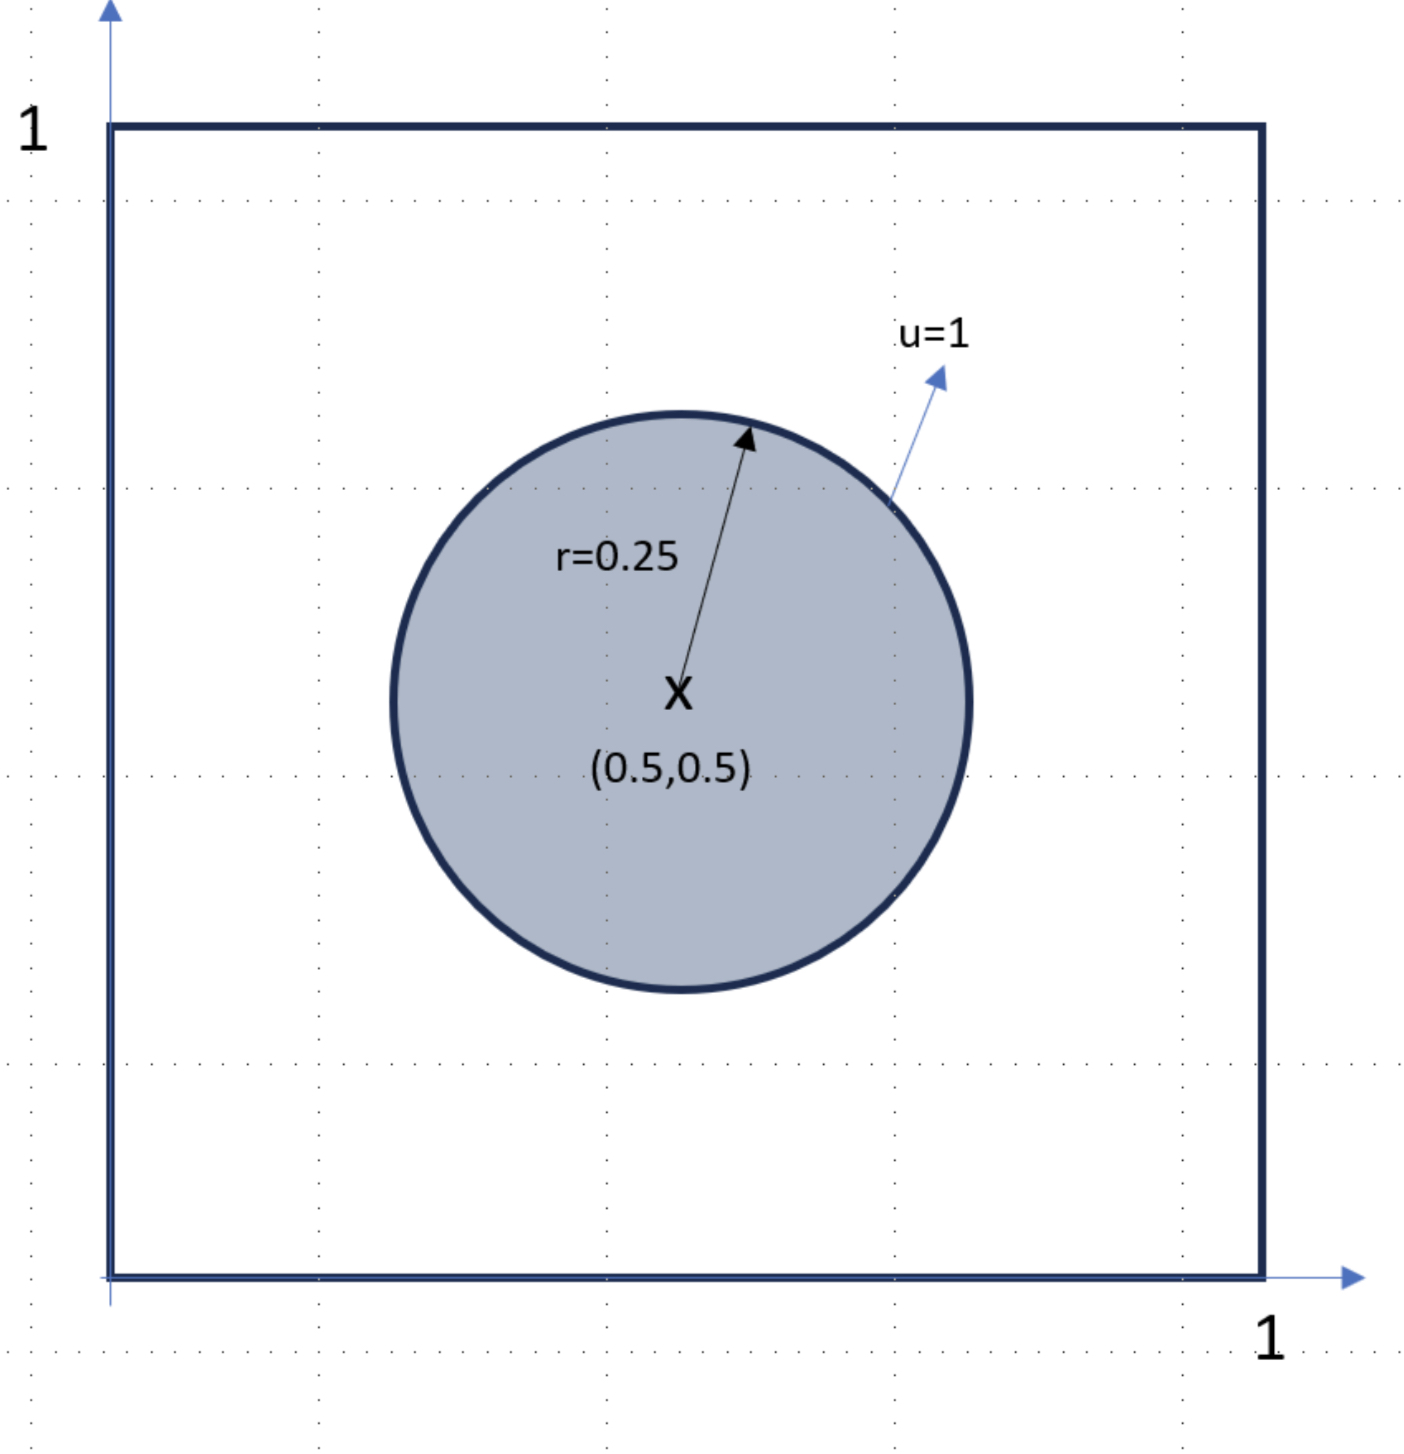
\includegraphics[width=0.4\textwidth]{Problem01.jpg}
    \caption{The domain with boundary conditions.}
\end{figure}

\noindent\textbf{(a)} Use a second-order central-difference scheme to develop an 
iterative solver to solve the above problem. Use the stair-step method to implement 
the boundary conditions on the internal boundary. Use point Gauss-Seidel (GS) with 
Successive Over-Relaxation (SOR). Follow the algorithm shown in class.\\

\textbf{(b)} Draw a flowchart of your solver. [10 points]\\

\textbf{(c)} Solve the problem on grids with \( 32 \times 32 \), 
\( 96 \times 96 \), \( 160 \times 160 \) grid cells, and a 
\( 224 \times 224 \) grid also. Use a random number generator to generate 
the starting guess for the field in the range of \( [-1, +1] \). Plot the 
residual versus iteration index and the contour plots of the converged solution 
for each of the grids for overrelaxation parameter of 1.0. [140 Points]\\

\textbf{(d)} How can you check the correctness of your solution? Are there 
some symmetry lines in the solution where you can obtain an exact solution 
and compare it to the numerical solution? Is there a different boundary 
condition you could use on the outer boundary for which you could 
obtain an exact solution and then compare your numerical solution? [25 points]\\



\textbf{(e)} Discuss the observed performance of iterative solver for each grid simulated here. Consider questions like:
\begin{enumerate}
        \item How does the convergence change with overrelaxation parameter? What is the optimal value of this parameter? Does this optimal value change with grid size? [25 points]
        \item How does the CPU time increase with number of grid points? Is the expected trend observed? [25 points]
        \item Does your solution exhibit the expected second-order accuracy? [50 points]
\end{enumerate}

\textbf{(f)} Repeat (e) for the configuration below. Also comment on how the convergence and CPU time is different from that for the previous configuration. [100 Points]\\


\begin{figure}[ht!]
    \centering
    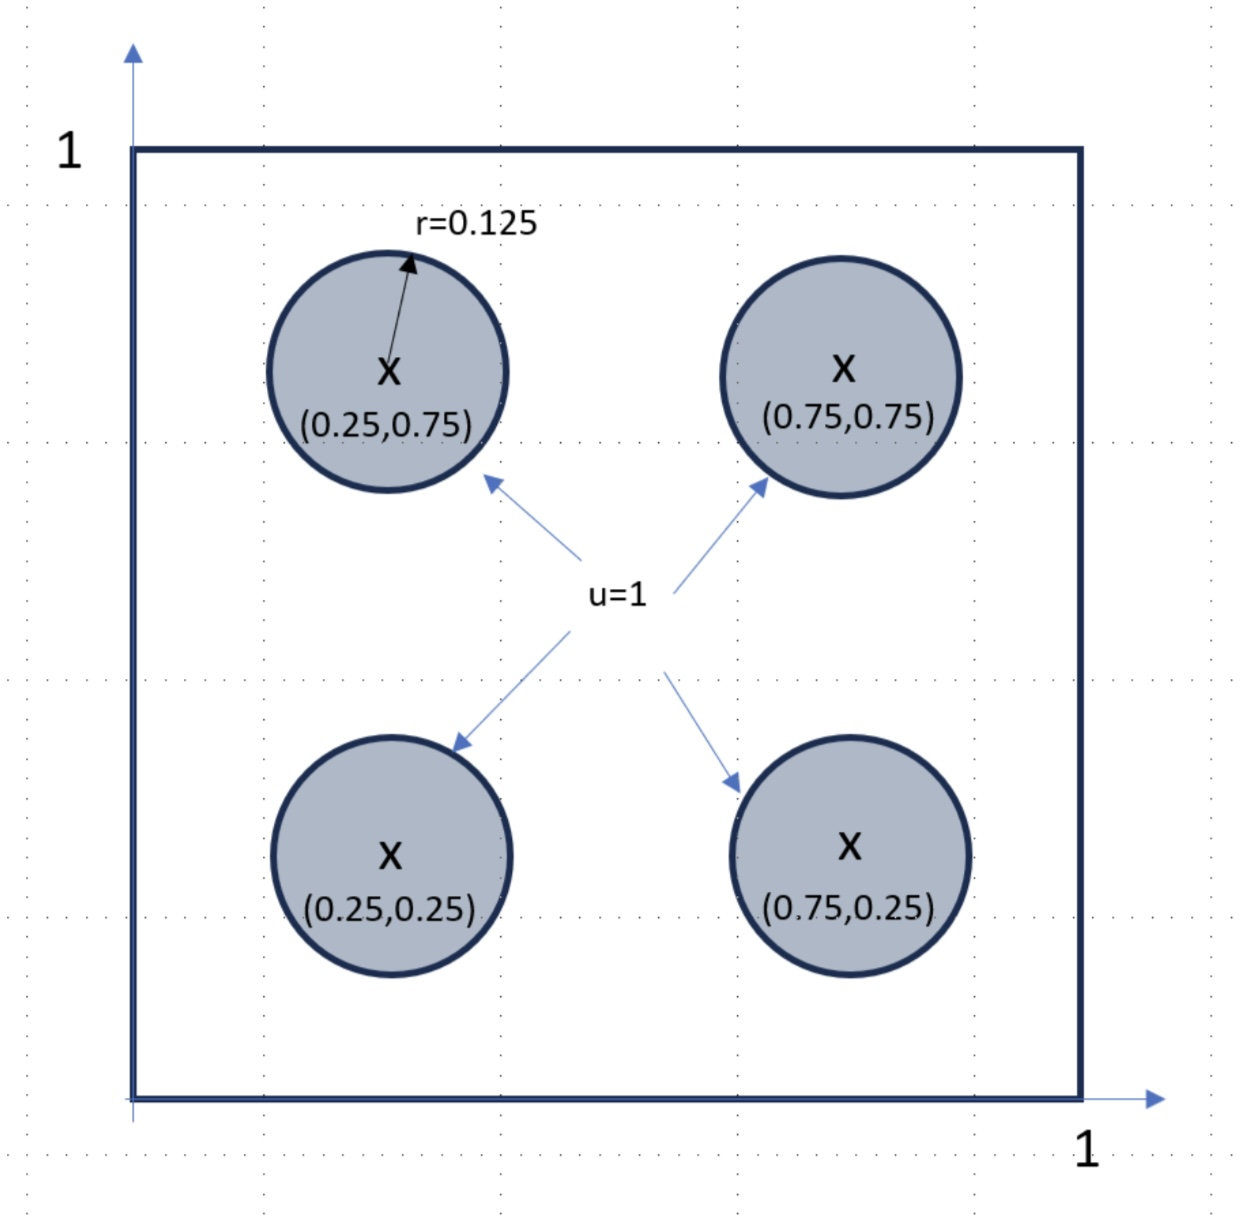
\includegraphics[width=0.4\textwidth]{Problem02.jpg}
    \caption{The domain with New boundary conditions.}
\end{figure}


\textbf{(g)} Solve the second configuration with Line-SOR and compare the convergence rate and CPU-time performance with point SOR. [75 points]\\

\textbf{(h)} \textbf{Challenge problem for extra points} -- Modify the solver to compute the potential flow past the 4-cylinder configuration in a much larger computational domain where you can impose free-stream conditions at the outer boundary. Plot streamlines and pressure contours of the flow. [50 points]\\

    








\section{(a) Iterative GS-SOR Solver}

\subsubsection{Grid Generator}
The first step to build a solver is to bulid is 
Grid Generator, whatever its boundary or platforms are.
Grid generstor's responsibility is to set platform with boundary,
which means it needs to:\\

(1) Create grid 

(2) identify points apply boundary condition

(3) identify points affected by boundary points directly 
(we call these Effected Points (EP))\\

According to our problem, identify part (2) need been done by ourself.
However, we need to solve inner boundary first.\\


Thus, we can divide our Grid Generator to three main functional
Creator: Grid-Creator, Inner Boundary Counter (IBcboundary), and 
Inner Boundary Conditionor (IBconditionor).

\paragraph{Grid-Creator}
For Grid-Creator, we just using the size of platform, and grid cell size.

\paragraph{Inner Boundary Counter (IBcboundary)}
For Inner Boundary Counter, the idea is using the formula of
inner Boundary, firstly to find the inner boundary limit in x and y 
direction.\\


In the limit, by using Stair-Step Method, for the real boundary intersected
whith horizontal line j (vertical coordinate), 
we can identify the i (horizontal coordinate)
for each Effective points.\\

Thus, we can find $i_{low}$ and $i_{high}$ for each j.

Similiar, we can find $j_{low}$ and $j_{high}$ for each i.\\



The simplest EPs can been divided by 4 kinds:\\

Boundary intersected with horizontal line(j line) on ($i_{low}$[j],j)

Boundary intersected with horizontal line(j line) on ($i_{high}$[j],j)

Boundary intersected with vertical line(i line) on (i,$j_{low}$[i])

Boundary intersected with vertical line(i line) on (i,$j_{high}$[i])\\


However, if just use these information, is hard to apply our control 
equation for th EPs, especially the formulas are different.\\

That's why we are going to transfor our information to 
Inner Boundary Classifier (IBclassfiier),
let it help us classify different kinds of EP points.\\

\paragraph{Inner Boundary Classifier (IBclassifier)}
We already get columns like $i_{low}$[j], this classifier is going to
generate conditions for each kind of EP:




\begin{figure}[H]
    \centering
    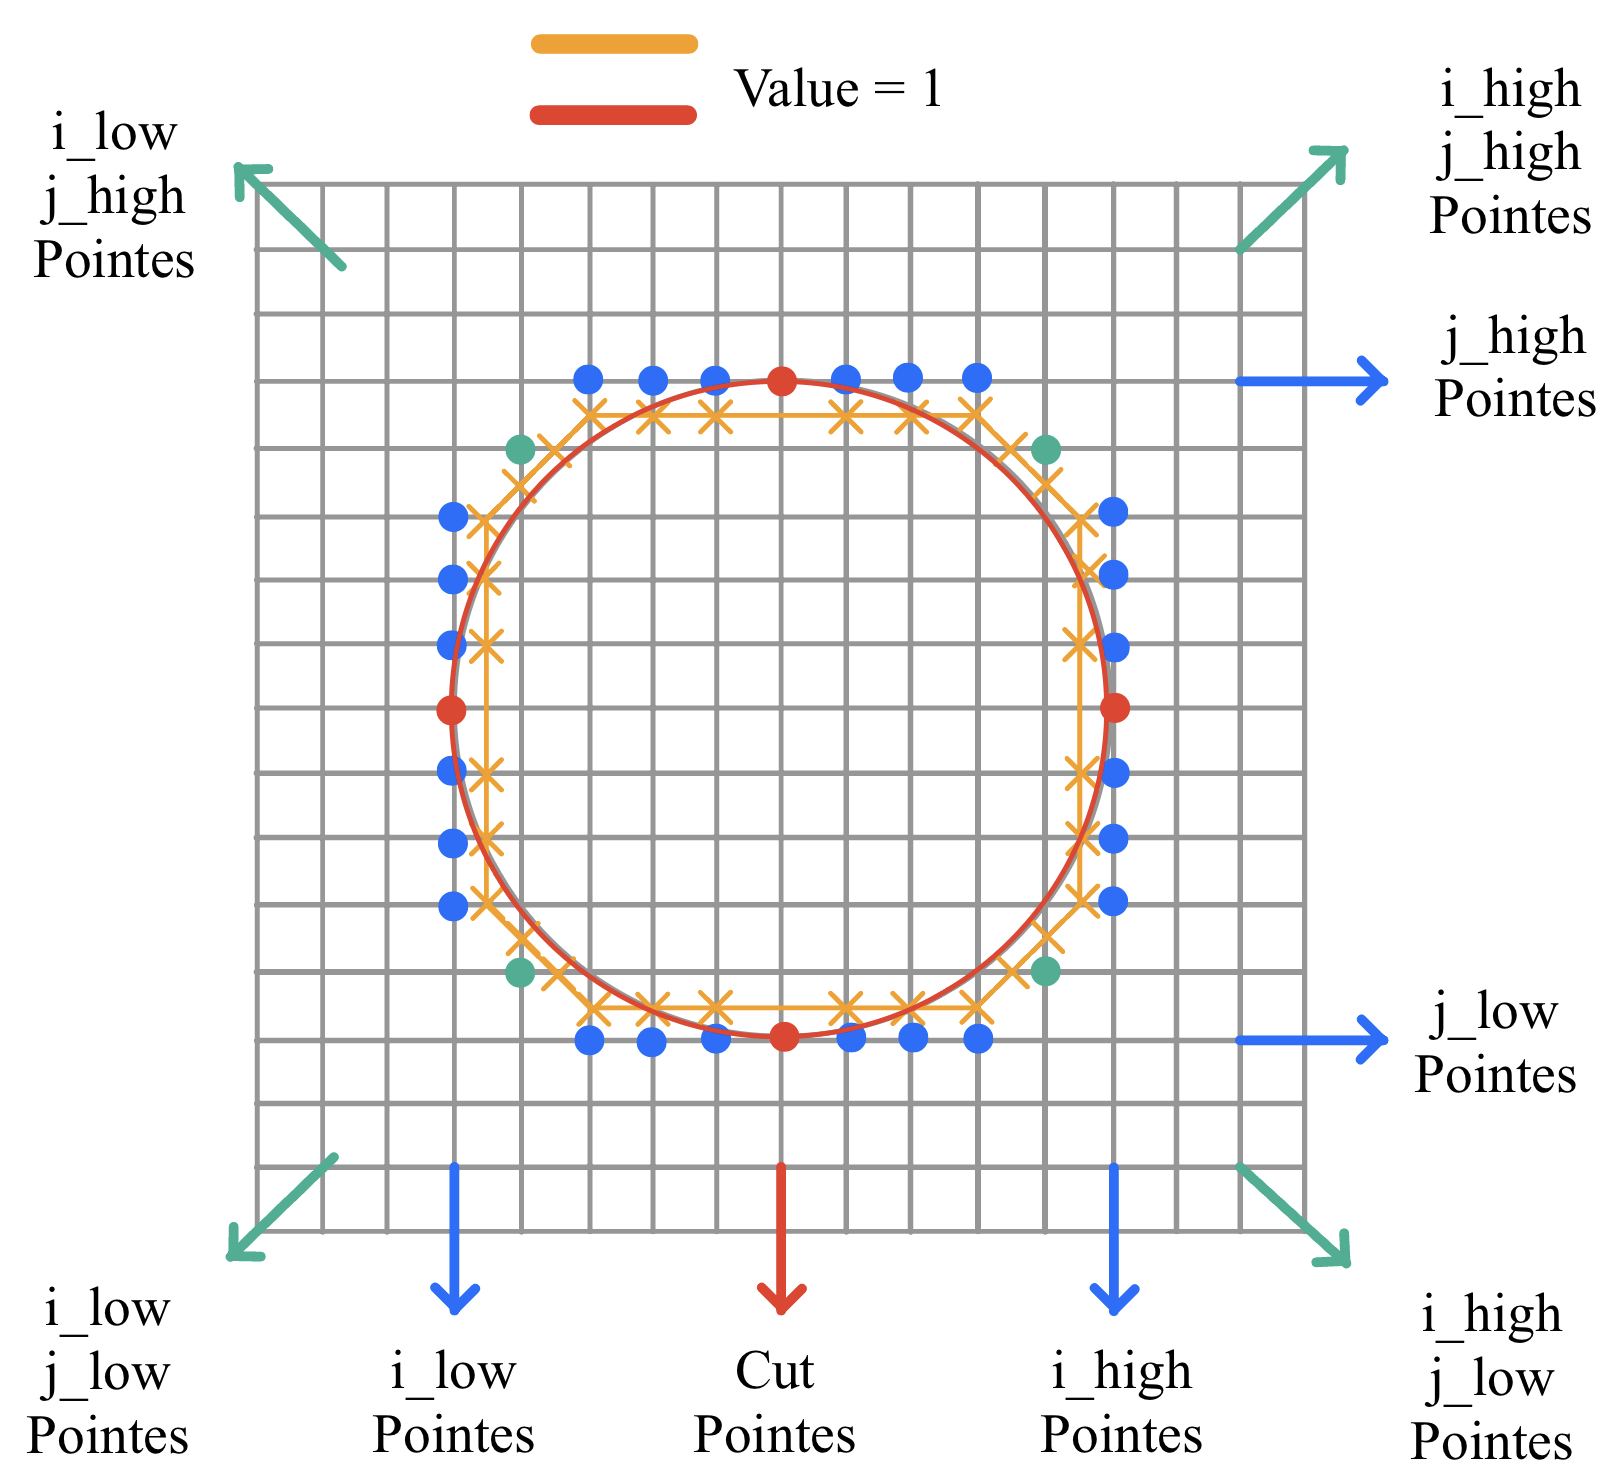
\includegraphics[width=0.7\textwidth]{Point_Classify.jpg}
    \label{Point_Classify.jpg    }
    \caption{Classify Different kinds of Effected Points}
\end{figure}


In this diagram, the Red line is circle boundary, while it cut through
grids, we use the orange line at each half grid as its step boundary, 
where is value equal to 1.\\

However, when we employ this method in to solver, what we calculate is 
not the orange lines directly, we calculate the bule and green points,
applying boundary modified control equation to these points, to replace
the actual boundary effect. These points we called Effected Points.
The Effected Points could be classified into 9 groups:\\

Blue:

(1) $i_{low}$: circle boundary only cuts grid at x-low lines.

(2) $i_{high}$: circle boundary only cuts grid at x-high lines.

(3) $j_{low}$: circle boundary only cuts grid at y-low lines.

(4) $j_{high}$: circle boundary only cuts grid at y-high lines.\\


Green:

(5) $i_{low\_j\_low}$: circle boundary cuts grid 
at x-low lines and y-low lines.

(6) $i_{low\_j\_high}$: circle boundary cuts grid 
at x-low lines and y-high lines.

(7) $i_{high\_j\_low}$: circle boundary cuts grid 
at x-high lines and y-low lines.

(8) $i_{high\_j\_high}$: circle boundary cuts grid 
at x-high lines and y-high lines.\\

Red:

(9) Cut Points: Where circle cut grid at grid points, Value=1\\



The iteration formula for these special points is showing below:\\

For $i_{low}$, we have:

\[ U_{xx} = \frac{4}{3\Delta^2} U_{i-1} - \frac{4}{\Delta^2} U_{i} + \frac{8}{3\Delta^2}  \]

Then, the iteration formula for $i_{low}$ is:

\[ U_i = \frac{1}{6} \left[ \frac{4}{3} U_{i-1,j} + \frac{8}{3}+ U_{i,j-1} + U_{i,j+1} \right] \]\\

For $i_{high}$, we have:
\[ U_{xx} = \frac{4}{3\Delta^2} U_{i+1} - \frac{4}{\Delta^2} U_{i} + \frac{8}{3\Delta^2}  \]

\[ U_i = \frac{1}{6} \left[ \frac{4}{3} U_{i+1,j} + \frac{8}{3}+ U_{i,j-1} + U_{i,j+1} \right] \]

Similarly, for For $j_{low}$::
\[ U_i = \frac{1}{6} \left[ \frac{4}{3} U_{i,j-1} + \frac{8}{3}+ U_{i-1,j} + U_{i+1,j} \right] \]

Similarly, for For $j_{high}$::
\[ U_i = \frac{1}{6} \left[ \frac{4}{3} U_{i,j+1} + \frac{8}{3}+ U_{i-1,j} + U_{i+1,j} \right] \]

Similarly, for $i_{low\_j\_low}$:
\[ U_i = \frac{1}{8} \left[ \frac{4}{3} U_{i-1,j} + \frac{4}{3} U_{i,j-1} + \frac{16}{3} \right] \]

Similarly, for $i_{low\_j\_high}$:
\[ U_i = \frac{1}{8} \left[ \frac{4}{3}U_{i-1,j} + \frac{4}{3} U_{i,j+1} + \frac{16}{3} \right] \]

Similarly, for $i_{high\_j\_low}$:
\[ U_i = \frac{1}{8} \left[ \frac{4}{3} U_{i+1,j} + \frac{4}{3} U_{i,j-1} + \frac{16}{3} \right] \]

Similarly, for $i_{high\_j\_high}$:
\[ U_i = \frac{1}{8} \left[ \frac{4}{3} U_{i+1,j} + \frac{4}{3} U_{i,j+1} + \frac{16}{3}  \right] \]


\subsubsection{Iteration Formula}
For General Point's calculation, the formula is showing below:

\begin{equation*}
    (u_{xx} + u_{yy}) = 0 \quad \text{for } 0 < x,y < 2\pi
\end{equation*}

Or in other notation: $$\nabla^2 P = 0 \quad $$


Add sudo-time part, obtain:
$$\nabla^2 P = \frac{\partial P}{\partial t}$$


Where is also can be shown as: 
\begin{equation*}
    (u_{xx} + u_{yy}) = u_{t} \\
\end{equation*}

Transfer Partial Difference Equartion (PDE) to Finite Difference equation
(FDE), use central difference method for spacial derivative transform, and
use forward difference for ``time" transformk, obtained:

\begin{align*}
    \frac{P_{ij}^{k+1} - P_{ij}^k}{\Delta t} &= \frac{1}{\Delta^2} \left[ P_{i-1,j}^k + P_{i+1,j}^k + P_{i,j-1}^k + P_{i,j+1}^k - 4P_{ij}^k \right]
\end{align*}

For stability, in 1-D scheme, r =<1/2, in 2-D scheme, r =< 1/4.
To obatin the biggest dt, let r= 1/4, which is $\frac{\Delta t}{\Delta^2} = \frac{1}{4}$,
where the FDE transfer to:

\begin{align*}
    \quad P_{ij}^{k+1} &= \frac{1}{4} \left[ P_{i-1,j}^k + P_{i+1,j}^k + P_{i,j-1}^k + P_{i,j+1}^k \right]
\end{align*}

The formula shown above is Jacobi iteration method.
For Gauss Seidel method, the equation is showing below:

\begin{align*}
    \quad P_{ij}^{k+1} &= \frac{1}{4} \left[ P_{i-1,j}^{k+1} + P_{i+1,j}^k + P_{i,j-1}^{k+1} + P_{i,j+1}^k \right]
\end{align*}

For residual, it could be calculated by compare our simulation result with
the source term, which is 0 in this scenario:

\begin{align*}
    r^k &= \frac{1}{\Delta^2} \left[ P_{i-1,j}^k + P_{i+1,j}^k + P_{i,j-1}^k + P_{i,j+1}^k - 4P_{ij}^k \right]
\end{align*}





\subsection{Grid Generator}


The Grid Genersator's function is already been explained on the subsection before,
the flow chart of Grid Generator is showing below:


\begin{figure}[H]
    \centering
    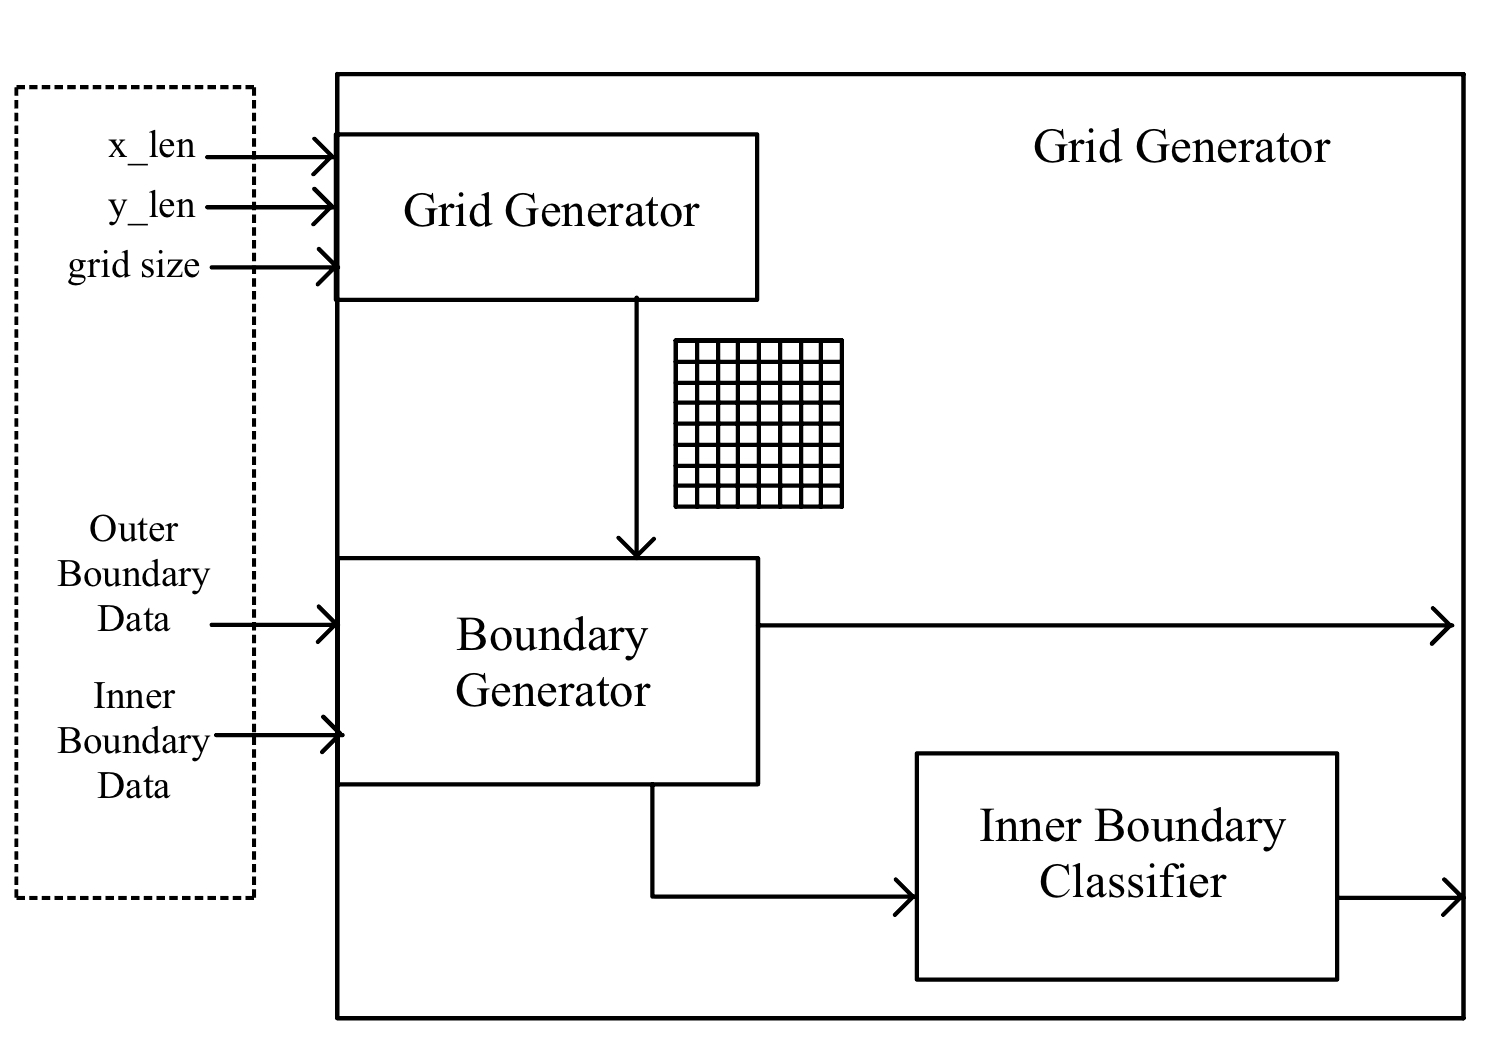
\includegraphics[width=0.6\textwidth]{Solver-Bg.jpg}
    \label{Grid Generator.jpg}
    \caption{Grid Generator}
\end{figure}





\subsection{Iteration Solver}




\begin{figure}[H]
    \centering
    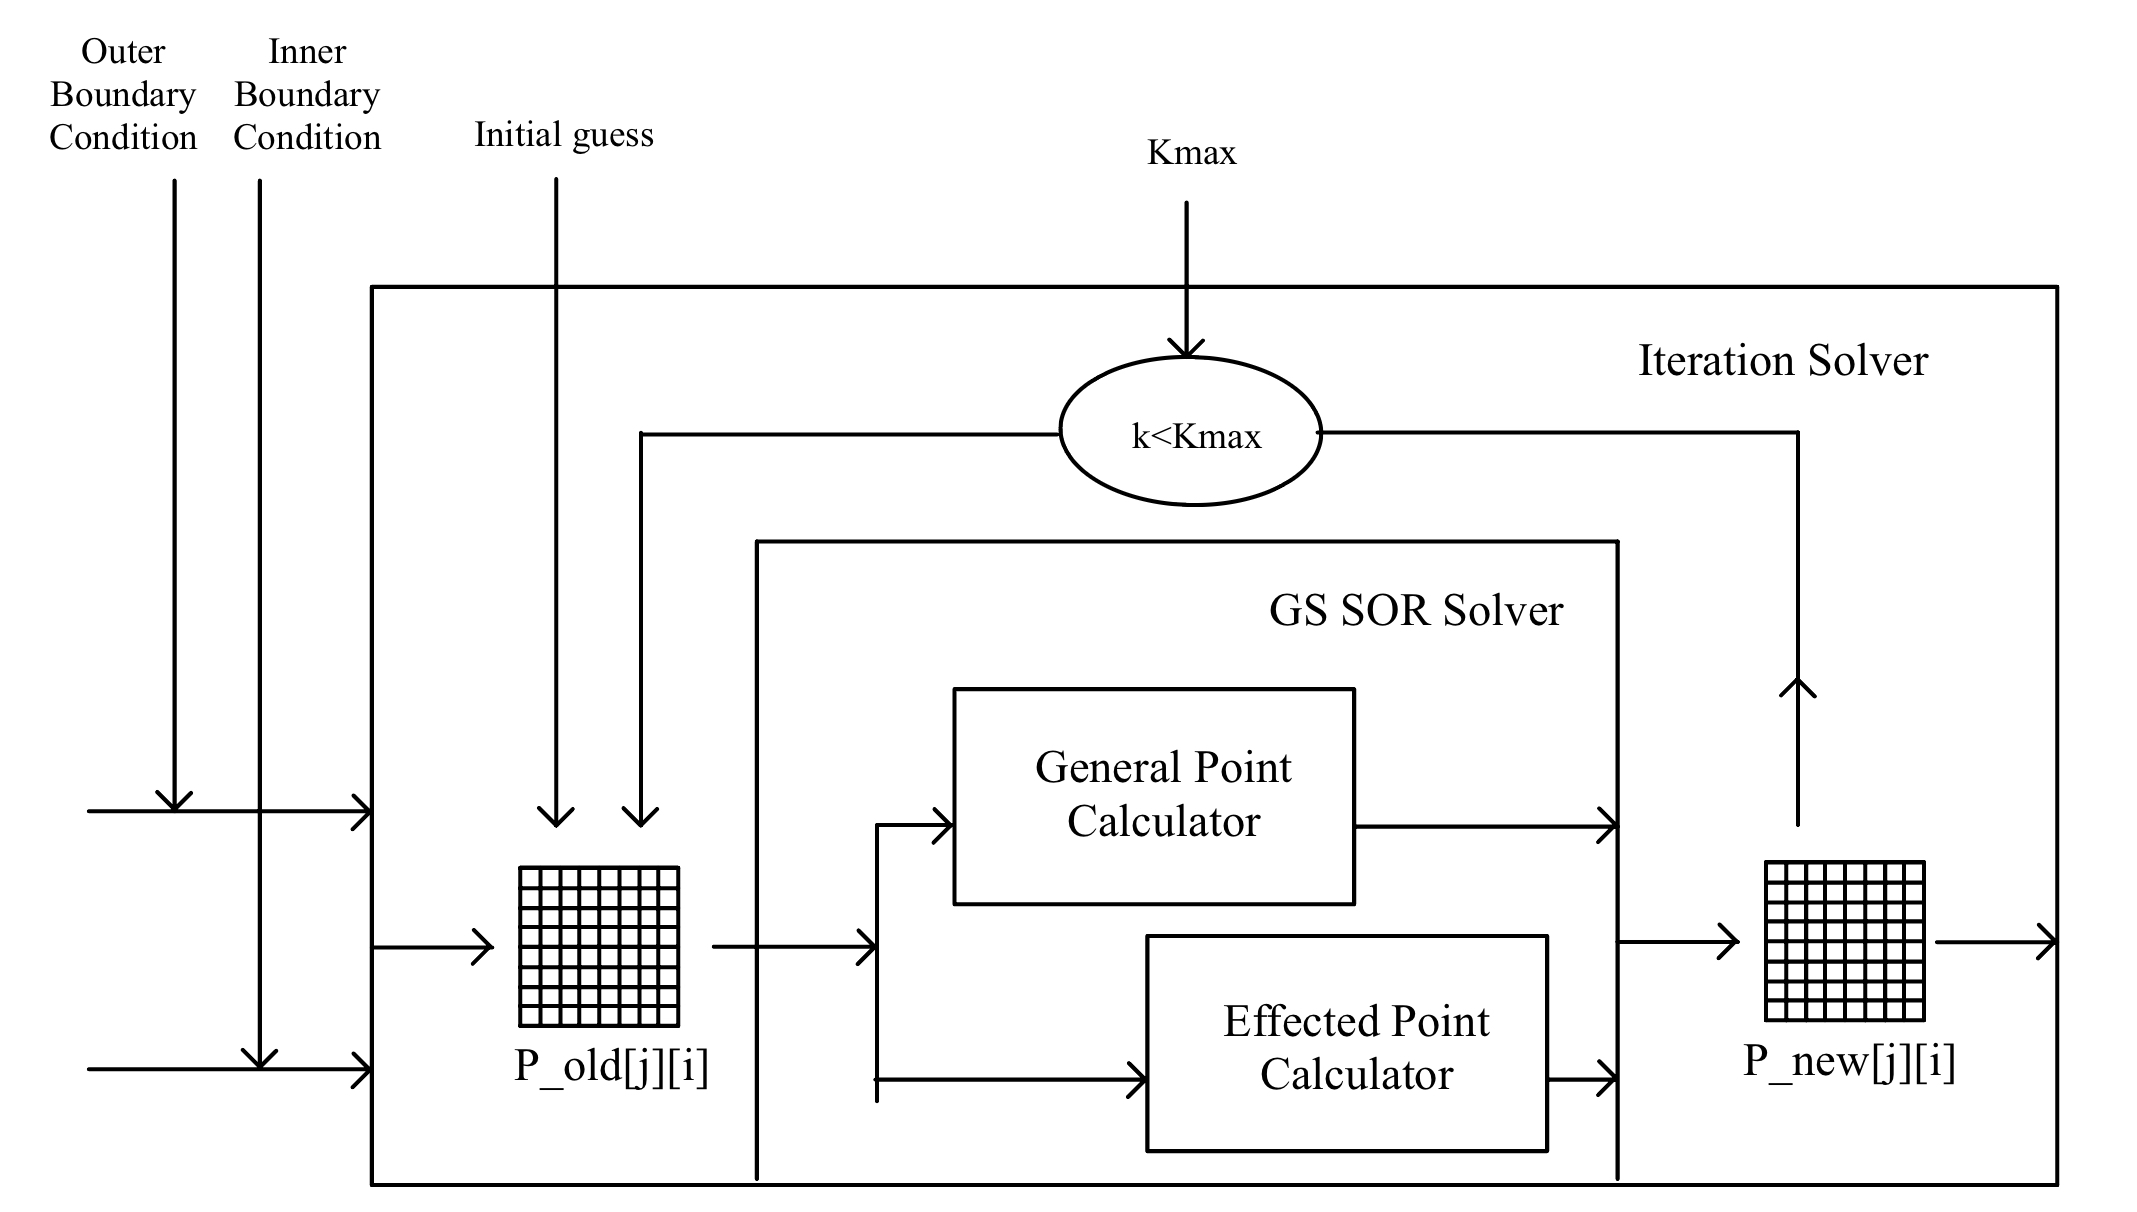
\includegraphics[width=0.8\textwidth]{Solver-It.jpg}
    \label{Grid Generator.jpg}
    \caption{Iteration Solver}
\end{figure}


The Sover diagram is showing above.
For iteration Solver, we already classified our points to General Points and 
Effected Points.


For General Points, the algorithm is showing below:

\begin{algorithm}
    \caption{Point Gauss-Seidel SOR Calculator}
    \begin{algorithmic}[1]
    \Procedure{Point\_GSSSOR}{$P_{\text{in}}, j_{\text{low}}, j_{\text{high}}, i_{\text{low}}, i_{\text{high}}, \omega$}
        \State $P_{\text{out}} \gets \text{deepcopy}(P_{\text{in}})$
        \For{$j \gets j_{\text{low}}$ to $j_{\text{high}}$}
            \For{$i \gets i_{\text{low}}$ to $i_{\text{high}}$}
                \State $P_{\text{out}}[j][i] \gets \frac{1}{4} \times (P_{\text{out}}[j][i-1] + P_{\text{out}}[j-1][i] + P_{\text{in}}[j][i+1] + P_{\text{in}}[j+1][i])$
                \State $P_{\text{out}}[j][i] \gets \omega \times P_{\text{out}}[j][i] + (1 - \omega) \times P_{\text{in}}[j][i]$
            \EndFor
        \EndFor
        \State \Return $P_{\text{out}}$
    \EndProcedure
    \end{algorithmic}
    \end{algorithm}

    For Effected Points, the algorithm is showing below:\\
    
    \begin{algorithm}
    \caption{Point Calculator for Effected Point using Gauss-Seidel SOR Method}
    \begin{algorithmic}[1]
    \Procedure{IBGSSOR}{$P_{\text{out}}, i, j, \omega, C_{\text{inner}}, C_{\text{total}}, C_{\text{xbl}}, C_{\text{ybl}}, C_{\text{ybh}}, C_{\text{edge}}, C_{\text{xyl}}, C_{\text{xyh}}, C_{\text{xyh}}$}
        \State $P_{\text{temp}} \gets \frac{1}{4} \left( P_{\text{out}}[i-1][j] + P_{\text{out}}[i][j-1] + P_{\text{in}}[i+1][j] + P_{\text{in}}[i][j+1] \right)$
        \State $P_{\text{corr}} \gets C_{\text{xbl}}[i][j] \times P_{\text{out}}[i-1][j] + C_{\text{ybl}}[i][j] \times P_{\text{out}}[i][j-1] + C_{\text{ybh}}[i][j] \times P_{\text{out}}[i+1][j] + C_{\text{edge}}[i][j] \times P_{\text{out}}[i][j+1]$
        \State $P_{\text{new}} \gets (1 - \omega) \times P_{\text{out}}[i][j] + \omega \times P_{\text{temp}} - \omega \times P_{\text{corr}}$
        \State $P_{\text{out}}[i][j] \gets P_{\text{new}}$
        \State \Return $P_{\text{out}}[i][j]$
    \EndProcedure
    \end{algorithmic}
    \end{algorithm}
    
C is the output of Inner Boundary Classifier, which value is 1 if the point we are 
using belong its class, the value become 0 if the point is not belong this class.

\subsection{Result Abnalysist}



\begin{figure}[H]
    \centering
    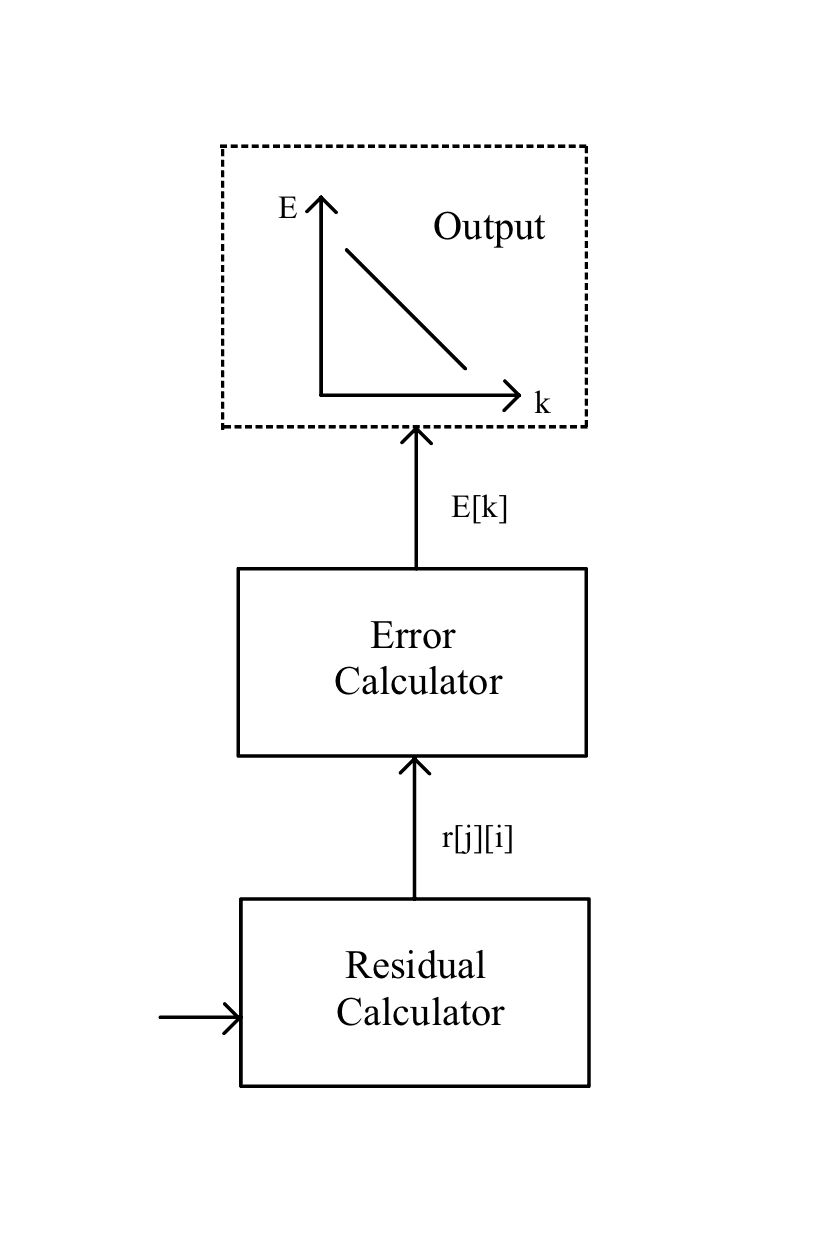
\includegraphics[width=0.3\textwidth]{Solver-Op.jpg}
    \label{Grid Generator.jpg}
    \caption{Result Analysist}
\end{figure}

The result analysist is going to capture each step's result, and calculate its
resuidual, then add the absolute resudial value at each point, find out the Error.
Then, it could plot the relationship of Error with iteration step.







\section{(b) Solver General Strture}
The whole solver diagram is showing below:


\begin{figure}[H]
    \centering
    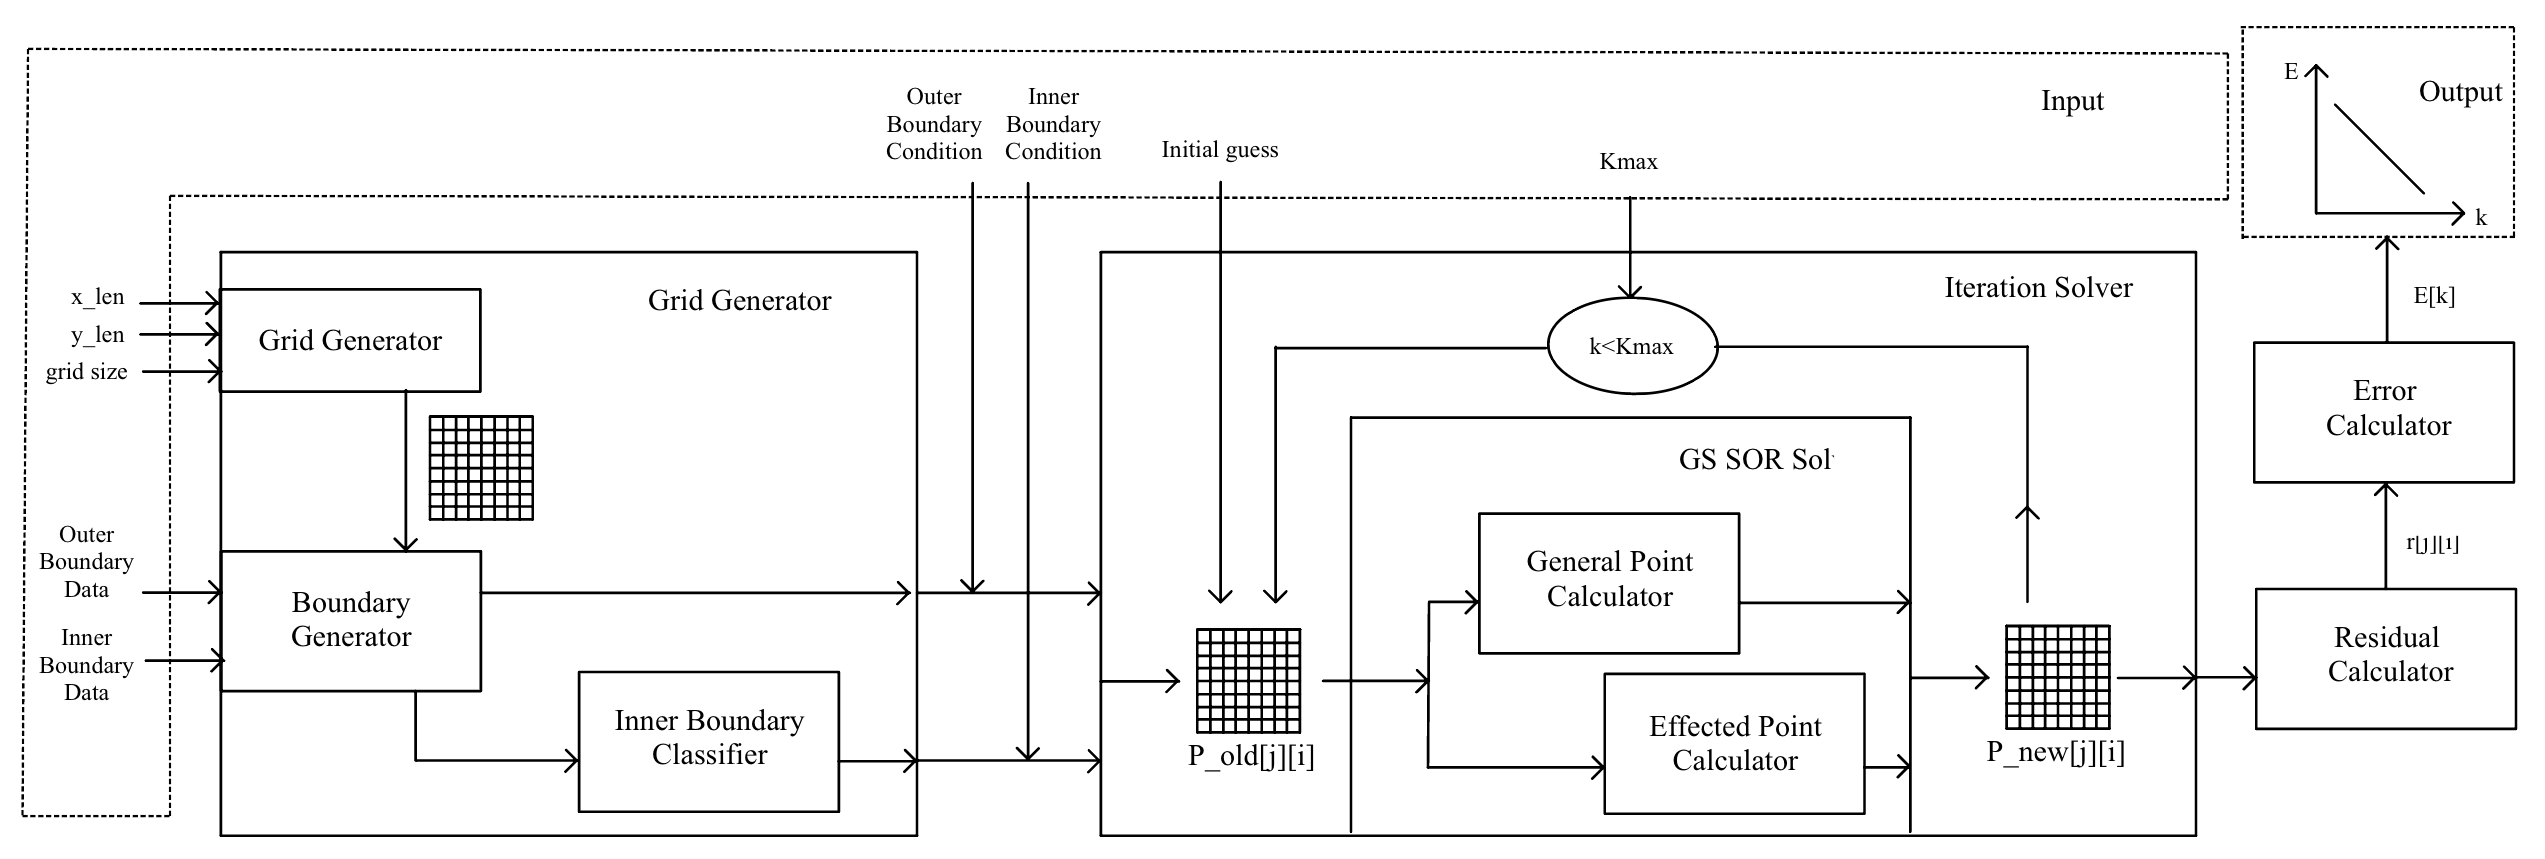
\includegraphics[width=1.1\textwidth]{Solver_Diagram.jpg}
    \label{Solver_Diagram.jpg}
    \caption{The Solver Diagram}
\end{figure}

As we can see, the Grid Geenrator generate grids and classify points to General Points
(GP) and Effected Points (GP, though it also need to classify EP again), then 
pass their data to Iteration Solver. The GS SOR Solver use their classification to 
calculate each points, and pass their new value back and calculate them again, 
until iteration number k reach Kmax. At each iteration step, Iteration Solver pass
the data to Result Analysist, and let it to calculate the residual of our 
Finite Difference Equation with Partial Difference Equation.



\section{(c) Iteration for different grid sizes}


Deploy our solver to solve this problem under control 2nd Laplace equation
and boundary condition, the result is showing below:

\subsection{Result Compare for each grid size}


Apply our solver to 32x32, 96x96, 160x160, and 224x224 grid size, the result is showing
below:



\begin{figure}[H]
    \centering
    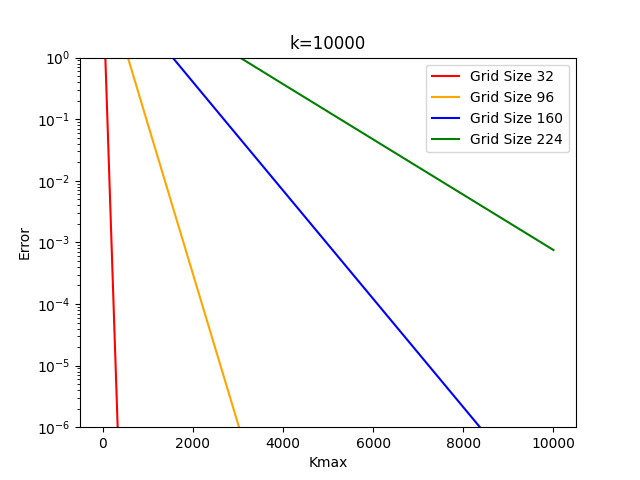
\includegraphics[width=0.9\textwidth]{Cnvergence4grids.png}
    \label{Cnvergence4grids.png}
    %\caption{Iteration times as k=200}
\end{figure}



\begin{figure}[H]
    \centering
    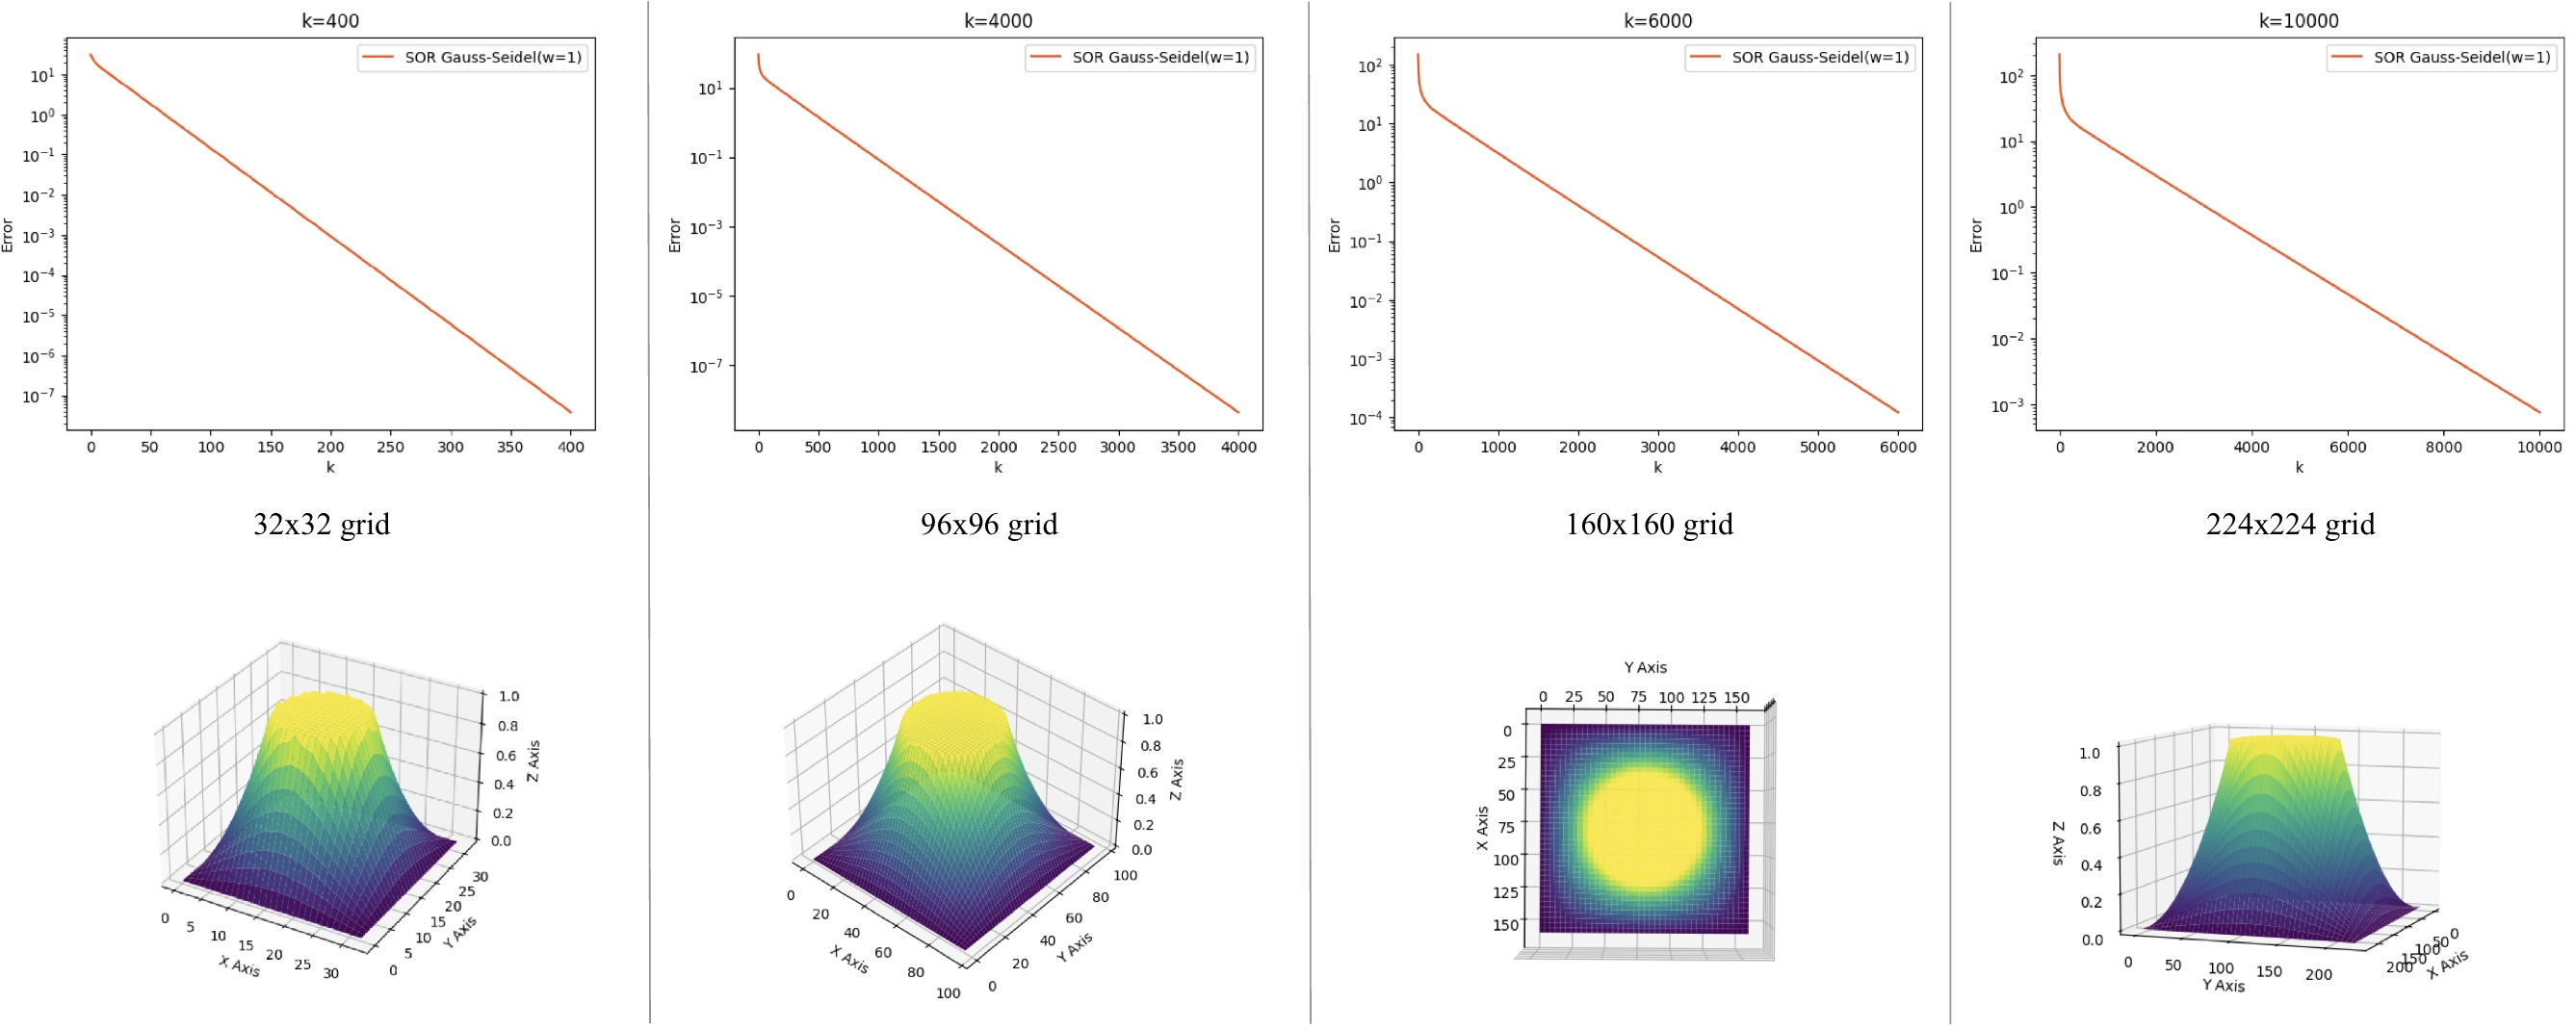
\includegraphics[width=1\textwidth]{(a)showall.jpg}
    \label{(a)showall.jpg}
    %\caption{Iteration times as k=200}
\end{figure}



It could be seen although in different size grid, the results are
similiar as its convergence trends are almost same
(except the convergnece rate), which keeping decreasing almost like
stright line at semi-log plot. Their final temperature distribution
are similiar, which could be seen at secnd row of the diagram,
that the highest temperature appear at the inner boundary, and 
show non-linear decrease characteristic at its path
reach the boundary.\\





\subsection{Result analysis}

\subsubsection{Need more iteration steps with fine grid}
For the result, we can see that as we are applying more fine grid,
the iteration steps we need is going to below up.\\

For 32x32 grid, it only need 200 iteration steps to obtain $10^{-3}$
accuracy, while it needs 2000 iteration steps for 96x96 gird,
and for 160x160 grid, is 4000 steps, for 224 grid, is 10000 steps to
reach $10^{-3}$ accuracy.

\subsubsection{Temperature distribution as expected}
We obtained two 3-D result for 32x32 grid at k=400, and also
for 96x96 grid at k=4000, the result are similiar,  fullfill
our expection: the temperature is high around inner boundary, and decrease
to zero as it reach outer boundary, the  distribution at this boundary 
condition is not linear at x or y direction.




\subsection{Detialed Result Show for each grid size}

\subsubsection{32x32 grid size}


\begin{figure}[H]
    \centering
    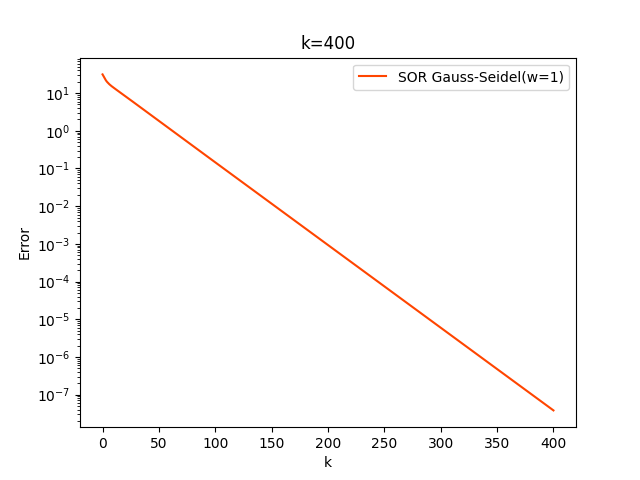
\includegraphics[width=0.6\textwidth]{aP=32.png}
    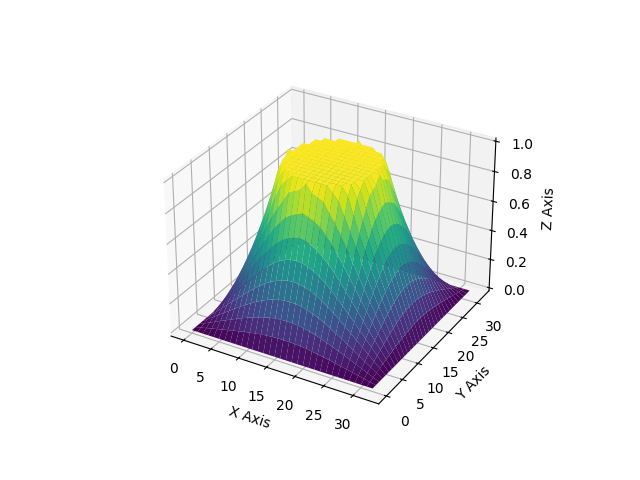
\includegraphics[width=0.38\textwidth]{32X32show.png}
    \label{aP=32.png}
    %\caption{Iteration times as k=200}
\end{figure}

For 32x32 size grid, it could be seen the error is decrasing fast at the semi-log 
plot, at iteration steps reach to 400, the error is already decrease to $10^{-7}$


\subsubsection{96x96 grid size}


\begin{figure}[H]
    \centering
    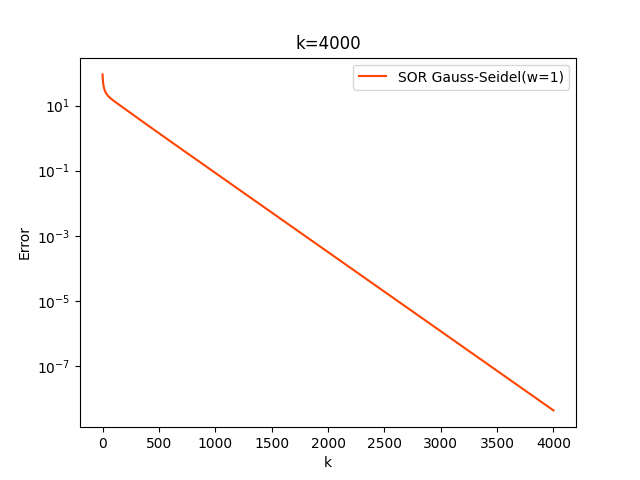
\includegraphics[width=0.6\textwidth]{aP=96.png}
    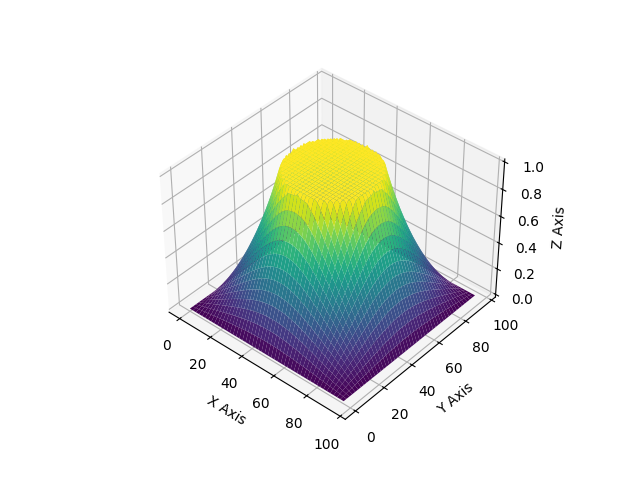
\includegraphics[width=0.38\textwidth]{96X96show.png}

    \label{aP=96.png}
    %\caption{Iteration times as k=200}
\end{figure}

For 96x96 grid size reuslt, we can see it is similiar to 32x32 sized grid.
However, its convergence much slower.



\subsubsection{160x160 grid size}


\begin{figure}[H]
    \centering
    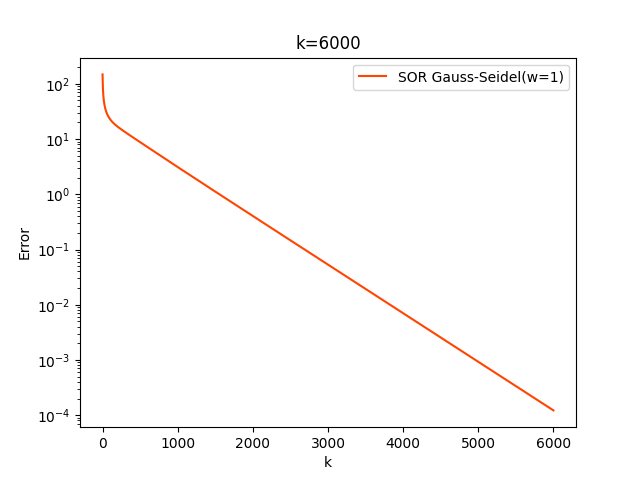
\includegraphics[width=0.8\textwidth]{aP=160.png}
    \label{aP=160.png}
    %\caption{Iteration times as k=200}
\end{figure}

We can see very similiar result with pervious results, that the convergence rate
now is also slower than 96x96 grid: the error only reach $10^{-4} $ as the iteration
steps already got to 6000.



The contour plot of 160x160 grid is showing below:
\begin{figure}[H]
    \centering
    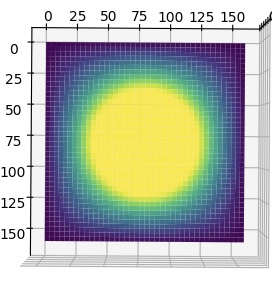
\includegraphics[width=0.4\textwidth]{grdi160show.jpg}
    \label{aP=160.png}
    \caption{Contour plot of 160x160 grid}
\end{figure}



\subsubsection{224x224 grid size}


\begin{figure}[H]
    \centering
    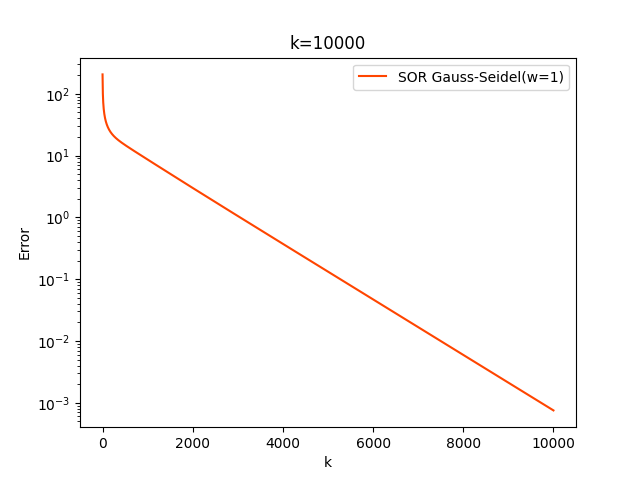
\includegraphics[width=0.8\textwidth]{aP=224.png}
    \label{aP=224.png}
    %\caption{Iteration times as k=200}
\end{figure}

For 224x224 grid, similiarly, it need 10000 iteration steps to let the error reach 
$10^{-3}$.


\section{(d) Check correctness of solution}

To check the correctness of the solution, it is obvious we cannot find symmetric lines
at this boundary condition. Thus, are going to obtain exact solution for another 
boundary condition where we can implement to our solve domain.


\subsection{Exact solution for circular outer boundary.}

The most simplest we we can see to obtain an exactsolution is to change the domain
from the square to a lrge circle, where the old square domain's four edges at this 
circle. Let this big circle be the outer domain edge, and let outer boundary
codition to u=0, we can obtain exact solution.\\



\begin{figure}[H]
    \centering
    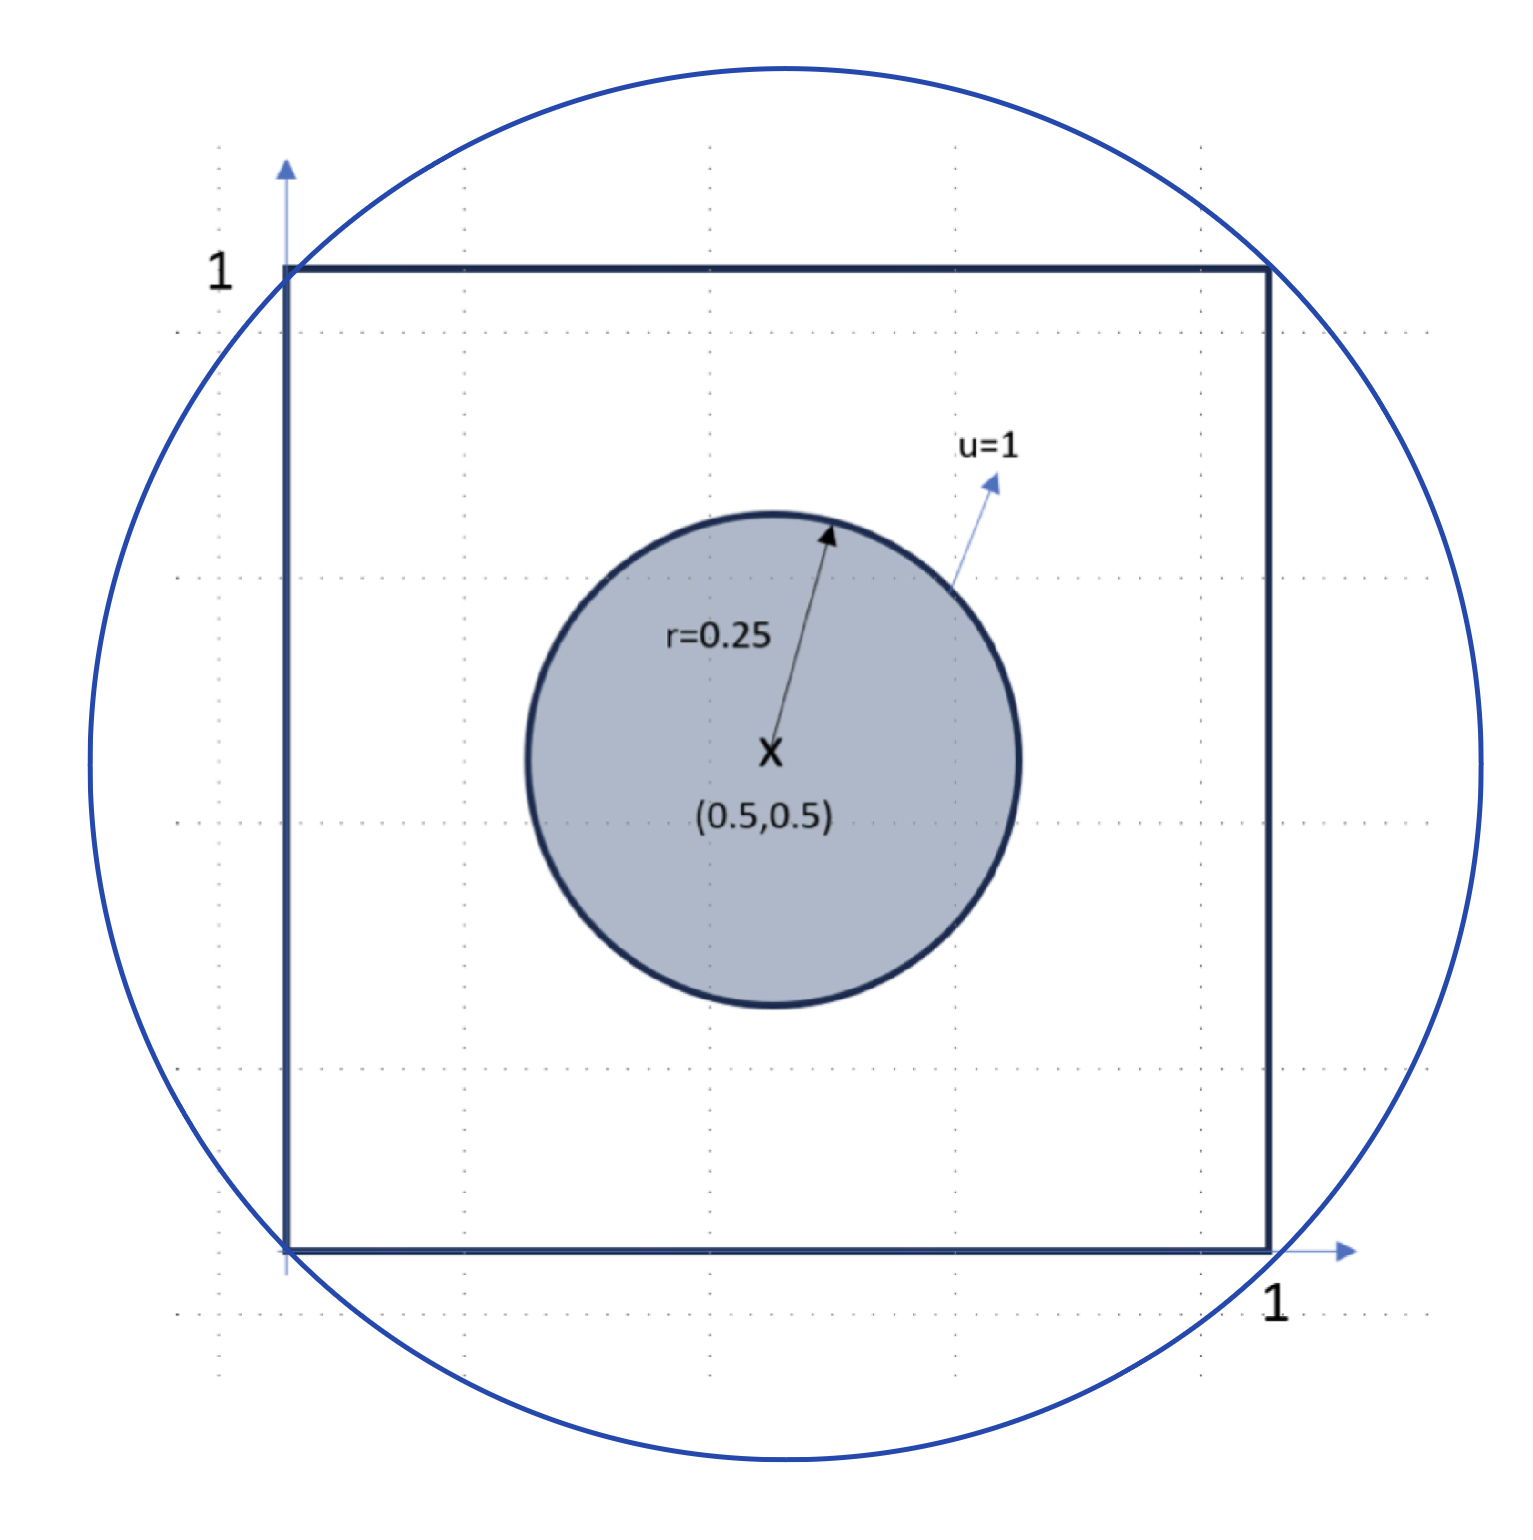
\includegraphics[width=0.4\textwidth]{ExactDomain.jpg}
    \label{ExactDomain.jpg}
    %\caption{Iteration times as k=200}
\end{figure}





\subsubsection{Exact solution}


Transfer control equation to polar coordinate:

\begin{equation}
    \frac{1}{r} \frac{\partial}{\partial r} \left( r \frac{\partial \Phi}{\partial r} \right) + \frac{1}{r^2} \frac{\partial^2 \Phi}{\partial \theta^2} = 0 \\
\end{equation}

By symmetric, we know $$\frac{\partial^2 \Phi}{\partial \theta^2} = 0$$

Thus, the equation becomes
\begin{equation}
    \frac{1}{r} \frac{\partial}{\partial r} \left( r \frac{\partial \Phi}{\partial r} \right) = 0 \\
\end{equation}



The solution of the equation is showing below:

\begin{equation}
    \Phi = C \ln r + C_2
\end{equation}



Apply boundary condition:

\begin{align*}
    \Phi \bigg|_{r=R_1} &= 1: \quad 1 = C \ln R_1 + C_2 \\
    \Phi \bigg|_{r=R_2} &= 0: \quad 0 = C \ln R_2 + C_2 \\
\end{align*}

The result is showing below:

\begin{equation}
    \Phi = \frac{\ln(r/R_2)}{\ln(R_1/R_2)} 
\end{equation}

Where $R_1$ is cylinder radius (=0.25), $R_2$ is outer domain boundary radius 
(=$\sqrt{2}$).


\subsubsection{Apply to numerical boundary}
The second step is to use our exact solution at our square boundary to change the 
old boubdary condition. As we know, the coordinate transfer at the boubdary:


\[
r = \sqrt{\left(\frac{a}{2}\right)^2 + \left(a - x\right)^2}
\]

Then, we could obtain our new boundary comdition:

\[
\Phi_{BC} = -\frac{\ln\left(\frac{a^2}{4} - ax + x^2\right)}{5 \ln 2}
\]

\[
a = 1: \quad \Phi_{BC} = -\frac{\ln\left(x^2 - x + 1\right)}{5 \ln 2}
\]


By applying this 'exact' boundary condition to our new outer boundary contition, 
the result form our solver is showing below:

\begin{figure}[H]
    \centering
    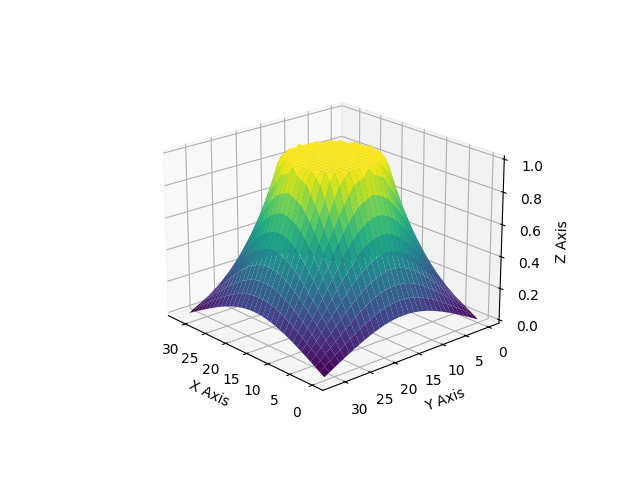
\includegraphics[width=0.6\textwidth]{WithExactB.png}
    \label{WithExactB.png}
    %\caption{Iteration times as k=200}
\end{figure}


\subsubsection{Result and analysis}



\begin{figure}[H]
    \centering
    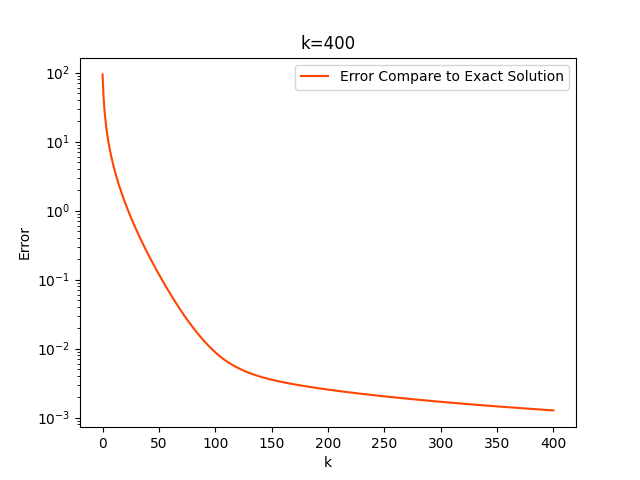
\includegraphics[width=0.6\textwidth]{ErrorwithExact.png}
    \label{ErrorwithExact.png}
    %\caption{Iteration times as k=200}
\end{figure}

It could be seen the error becomes much slower as the iteration going, it could say 
our simulation is correct, the exactness will be pretty good as iteration going.















\section{(e) Solver Performance Check}
\subsection{(I) Overrelaxation Parameter}
For each grid, we test our overrelaxation parameter from in the range of [1,2], 
step size=0.1, the change with overrelaxation parameter with its convergence speed
is showing below:

\begin{figure}[H]
    \centering
    % 第一行的两张图片
    \begin{minipage}{0.45\textwidth}
        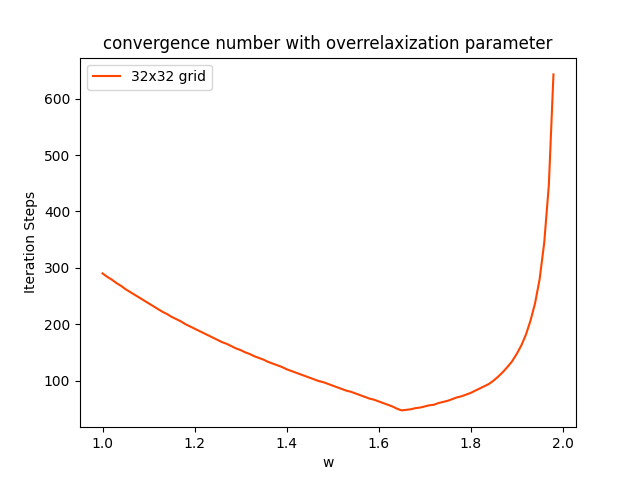
\includegraphics[width=\linewidth]{ws_for32grid.png}
        \caption{32x32 grid}
        \label{fig:32grid}
    \end{minipage}
    \hfill
    \begin{minipage}{0.45\textwidth}
        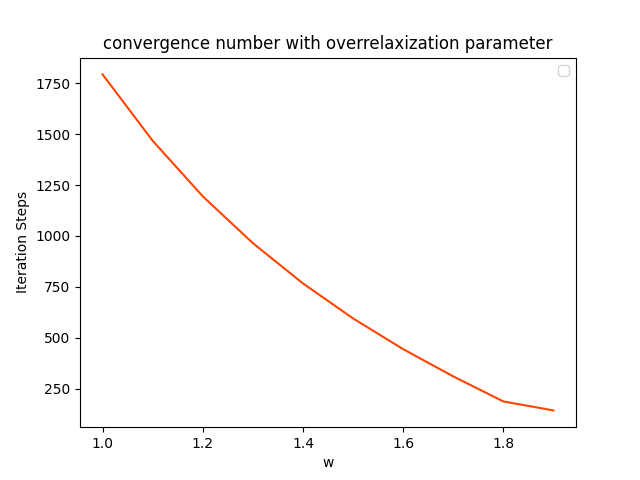
\includegraphics[width=\linewidth]{0.01ws_for96grid.png}
        \caption{96x96 grid}
        \label{fig:96grid}
    \end{minipage}

    \vspace{1em} % Adds some space before the next row

    % 第二行的两张图片
    \begin{minipage}{0.45\textwidth}
        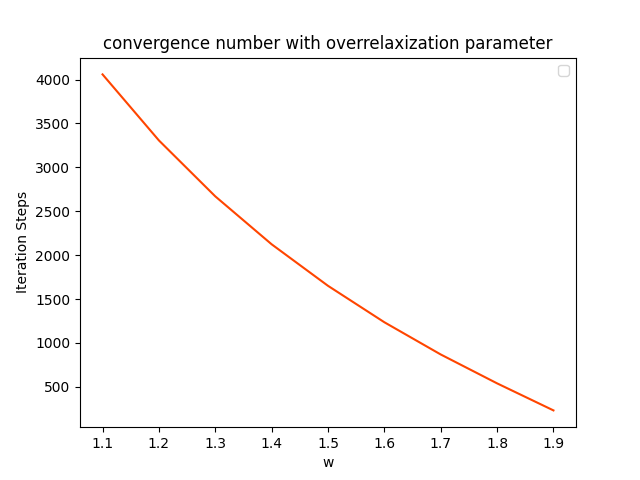
\includegraphics[width=\linewidth]{0.1ws_for160grid.png}
        \caption{160x160 grid}
        \label{fig:160grid}
    \end{minipage}
    \hfill
    \begin{minipage}{0.45\textwidth}
        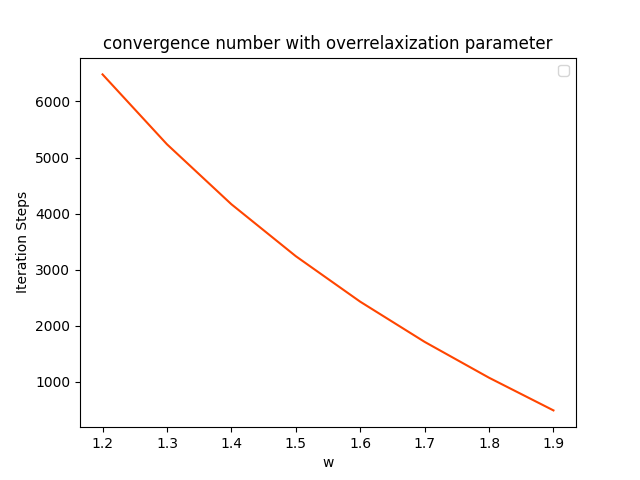
\includegraphics[width=\linewidth]{0.1wsfor224grid.png}
        \caption{224x224 grid}
        \label{fig:224grid}
    \end{minipage}

    % 总标题
    \caption{Accuracy diagrams for different grid sizes.}
    \label{fig:grids}
\end{figure}



\begin{table}[ht]
    \centering
    \begin{tabular}{cccccccccccc}
    \toprule
    Size $\backslash$ w & 1.0 & 1.1 & 1.2 & 1.3 & 1.4 & 1.5 & 1.6 & 1.7 & 1.8 & 1.9 & 2.0 \\
    \midrule
    32 grid & 199 & 163 & 132 & 106 & 83 & 63 & 45 & \textbf{39} & 58 & 107 &\( K_{\text{max}} \) \\
    96 grid & 1794 & 1468 & 1195 & 965 & 767 & 595 & 444 & 310 & 187 & \textbf{143} & \( K_{\text{max}} \) \\
    160 grid & 6001 & 4059 & 3307 & 2670 & 2124 & 1651 & 1236 & 869 & 540 & \textbf{232} & \( K_{\text{max}} \) \\
    224 grid & \( K_{\text{max}} \) & \( K_{\text{max}} \) &  6843 & 5236 & 4166 & 3239 & 2427 & 1710 & 1070 & \textbf{487} & \( K_{\text{max}} \) \\
    \bottomrule
    \end{tabular}
    \caption{The iteration number to reach $10^{-3}$ Error with different ws}
    \label{tab:my_label}
\end{table}
    
    It could be found for 32 size grid, the optimal w is around 1.7, where for 
    96, 160, and 224 grid, the optimal w is around 1.9. It shows the finier the grid as,
    the more optimal overrelaxation parameter w move towards 2.


Consider the formula for Amplifaction factor:

\begin{equation}
G = \frac{1 - \omega + \frac{\omega}{2} e^{i k_x \Delta x}}
         {1 - \frac{\omega}{2} e^{-i k_x \Delta x}}
  = \frac{2 - 2\omega + \omega[\cos \beta_x + i \sin \beta_x]}
         {2 - \omega[\cos \beta_x - i \sin \beta_x]}
  = \frac{(2 - 2\omega + \omega \cos \beta_x) + i\omega \sin \beta_x}
         {2 - \omega \cos \beta_x + i\omega \sin \beta_x}
\end{equation}









\subsection{(II) CPU time}


For Error get $10^{-5}$, w =1, the CPU time for each method is showing below:


\begin{table}[ht]
    \centering
    \begin{tabular}{c|c | c | c}
    \hline
    Grid Size & CPU Time (seconds) & Iteration Steps (K) & Iteration Speed (it/s)\\ \hline
    32x32     & 0.9722             & 290                 & 305.96  \\ \hline
    96x96     & 70.5959            & 2616                & 35.32   \\ \hline
    160x160   & 561.3094           & 7234                & 12.89   \\ \hline
    320x320   & 2136.2018          & 14181               & 6.64    \\ \hline
    \end{tabular}
    \caption{CPU Time Till Convergnece for Different Grid Sizes}
    \label{tab:cpu_time}
\end{table}
    
It could be seen number iteration speed is have some relationship with grid size,
As the grid become finier, the iteration speed become much more slower, nearly
to $\text{Flop} =\sim N^{3}$



\subsection{(III) Order of accuracy}

The result shown 1st Order Accuracy for K=100:




\begin{figure}[H]
    \centering
    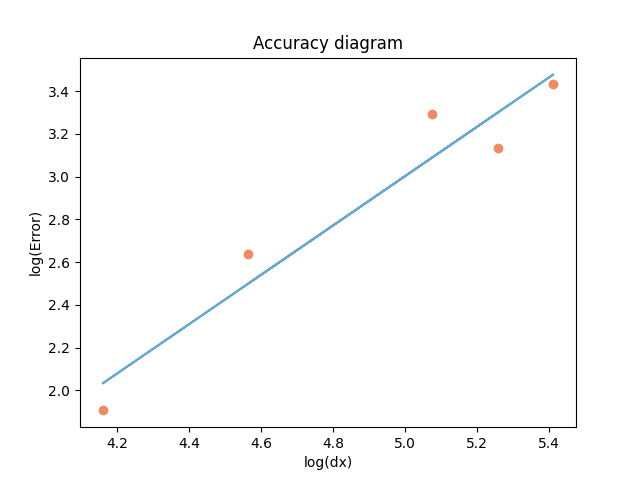
\includegraphics[width=0.7\textwidth]{orderofAccuracy.png}
    \label{orderofAccuracy.png}
    \caption{Order of Accuracy log-log}
\end{figure}


It could be see the slop is about 2, which means the error is 2nd order, this proves 
the method we are using (point GS-SOR) is second order accuracy.


\section{(f) 4-Cylinder Iteration Approach}

For 4-Cylinder Domain, adjust the inner boundary for the new condition, the grid 
generator for this step to generate 1-cylinder inner boundary first, and then 
duplicate to correspond coordinate. The rest for the solver is same.

The simulation for 4-cylinder condition is showing below:


\begin{figure}[H]
    \centering
    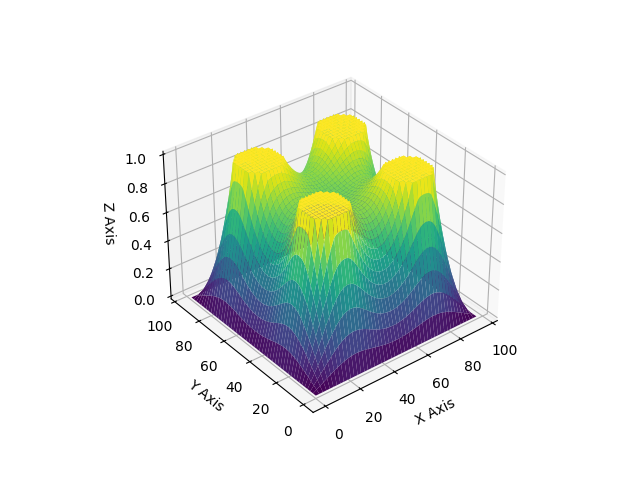
\includegraphics[width=0.7\textwidth]{4cylinder_simple_show.png}
    \label{4cylinder_simple_show.png}
    %\caption{Iteration times as k=200}
\end{figure}


\subsection{(I) Optimal overrelaxation parameter}

As we observed in the section (e), ther do exist optimal parameter w even can 
speed up 224 size grid from 10000 to 487, thus, this time we set up \( K_{\text{max}} \)
for only 1001, to find out optimal parameter for each grid, and speed up our program.

The result is showing below:


\begin{table}[ht]
    \centering
    \begin{tabular}{cccccccccccc}
    \toprule
    Size $\backslash$ w & 1.0 & 1.1 & 1.2 & 1.3 & 1.4 & 1.5 & 1.6 & 1.7 & 1.8 & 1.9 & 2.0 \\
    \midrule
    32 grid & 309 & 252 & 205 & 164 & 130 & 99 & 71 & \textbf{54} & 75 & 143 &  \( K_{\text{max}} \)   \\
    96 grid & \( K_{\text{max}} \) & \( K_{\text{max}} \) & \( K_{\text{max}} \) & \( K_{\text{max}} \) & \( K_{\text{max}} \) & 820 & 613 & 429 & 263 & \textbf{199} & \( K_{\text{max}} \) \\
    160 grid & \( K_{\text{max}} \) & \( K_{\text{max}} \) & \( K_{\text{max}} \) & \( K_{\text{max}} \) & \( K_{\text{max}} \) & \( K_{\text{max}} \) & \( K_{\text{max}} \) & \( K_{\text{max}} \) & 728 & \textbf{322} & \( K_{\text{max}} \) \\
    224 grid & \( K_{\text{max}} \) & \( K_{\text{max}} \) &  \( K_{\text{max}} \) & \( K_{\text{max}} \) & \( K_{\text{max}} \) & \( K_{\text{max}} \) & \( K_{\text{max}} \) & \( K_{\text{max}} \) & \( K_{\text{max}} \) & \textbf{656} & \( K_{\text{max}} \) \\
    \bottomrule
    \end{tabular}
    \caption{The iteration number to reach $10^{-3}$ Error with different ws}
    \label{tab:my_label}
\end{table}




Compare to our pervious 1-cylinder iteration, it could be seen as the boundary condition
brecome more complicated, the convergence rate decrease, while the optimal parameter
is almost in same condition: for 32 grid, is about 1.7, for others, is about 1.9.\\



The plot for each grid size is showing below:




\begin{figure}[H]
    \centering
    % 第一行的两张图片
    \begin{minipage}{0.45\textwidth}
        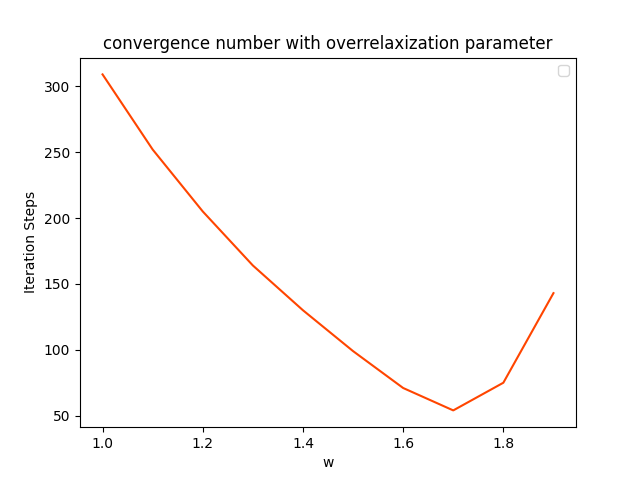
\includegraphics[width=\linewidth]{4cyws32.png}
        \caption{32x32 grid}
        \label{fig:32grid}
    \end{minipage}
    \hfill
    \begin{minipage}{0.45\textwidth}
        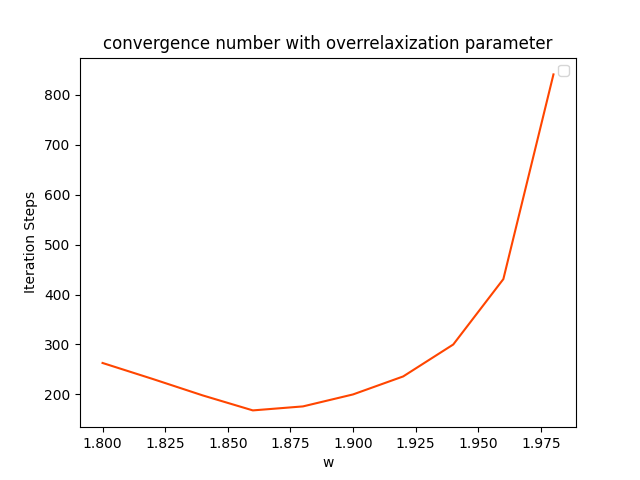
\includegraphics[width=\linewidth]{4cy96grid0.02w.png}
        \caption{96x96 grid}
        \label{fig:96grid}
    \end{minipage}

    \vspace{1em} % Adds some space before the next row

    % 第二行的两张图片
    \begin{minipage}{0.45\textwidth}
        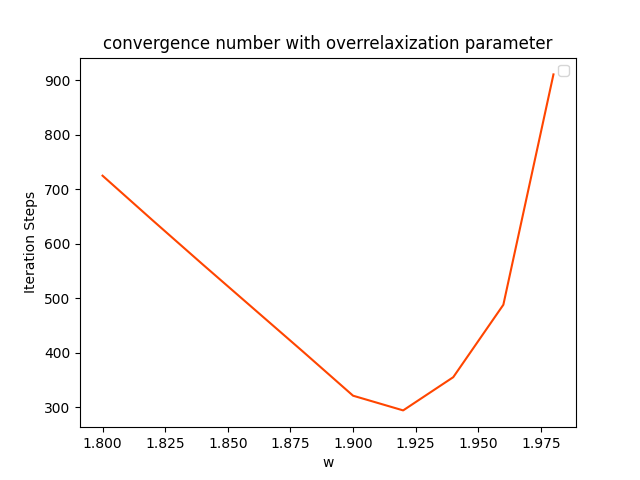
\includegraphics[width=\linewidth]{4cy160grid0.02w.png}
        \caption{160x160 grid}
        \label{fig:160grid}
    \end{minipage}
    \hfill
    \begin{minipage}{0.45\textwidth}
        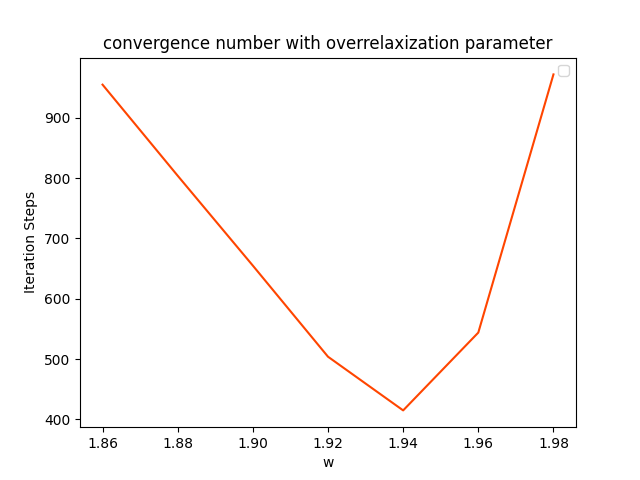
\includegraphics[width=\linewidth]{4cy224grid0.02w.png}
        \caption{224x224 grid}
        \label{fig:224grid}
    \end{minipage}

    % 总标题
    \caption{Accuracy diagrams for different grid sizes.}
    \label{fig:grids}
\end{figure}



For more detailized analysis, we try for 0.02 grid size for 95x96 grid, 160x160 grid,
and 224x224 grid, with w in range of [1.7, 2.0]

It could be seen, for 4 cylinder, w stepsize=0.02, the optimal overrelaxation
parameter for 96 grid is 1.86, which need 168 iteration to converge to $10^{-3}$.

The optimal value for 160 grid is 1.92, need 294 iterations to converge to $10^{-3}$.

For 224 grid, is 1.94, which repersent 415 iteration operations to decrease error
to $10^{-3}$.


    



\subsection{(II) CPU time}


For Error get $10^{-5}$, w =1, the CPU time for each method is showing below:


\begin{table}[ht]
    \centering
    \begin{tabular}{c|c | c | c}
    \hline
    Grid Size & CPU Time (seconds) & Iteration Steps (K) & Iteration Speed (it/s)\\ \hline
    32x32     & 1.1654             & 459                 & 410.28  \\ \hline
    96x96     & 70.5959            & 2616                & 35.32   \\ \hline
    160x160   & 561.3094           & 7234                & 12.89   \\ \hline
    320x320   & 2136.2018          & 14181               & 6.64    \\ \hline
    \end{tabular}
    \caption{CPU Time Till Convergnece for Different Grid Sizes}
    \label{tab:cpu_time}
\end{table}
    


\subsection{(III) Order of accuray}




\begin{figure}[H]
    \centering
    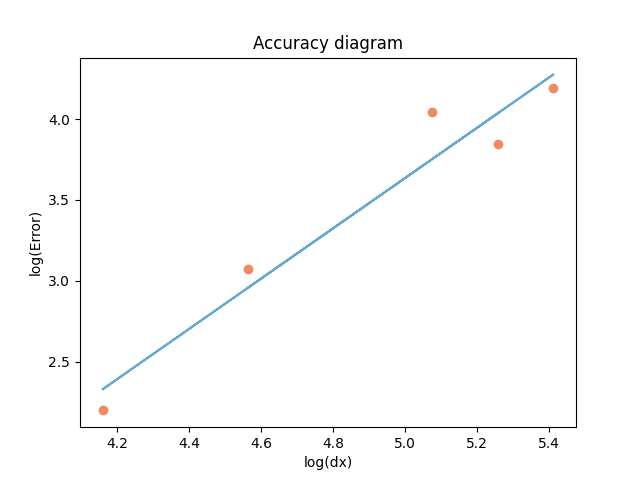
\includegraphics[width=0.7\textwidth]{4cyOrderofAccuracy.png}
    \label{4cyOrderofAccuracy.png}
    \caption{Order of Accuracy log-log}
\end{figure}

















\section{(g) Line-SOR Approach}
Apply Line SOR to our control equation, showing below:\\


(i) Line matrix operation


The control equation could be writen as discrete form:

\begin{equation*}
\left( \frac{\delta^2}{\Delta x^2} + \frac{\delta^2}{\Delta y^2} \right) u = S
\end{equation*}


Where, we apply line operation:

\begin{equation*}
\frac{\delta^2 u^{k+1}}{\Delta x^2} + \frac{\delta^2 u^k}{\Delta y^2} = S
\end{equation*}

k+1 is for the new value, where k means the old value, which we already known:


\begin{equation*}
u_{i,j}^{k+1} - 2u_{i,j}^{k+1} + u_{i+1,j}^{k+1} + u_{i,j-1}^{k} - 2u_{i,j}^{k+1} + u_{i,j+1}^{k} = S
\end{equation*}



(ii) SOR operation

\begin{equation*}
u^{k+1} = (1-\omega)u^k + \omega u^{*}
\end{equation*}

\begin{equation*}
u_{i,j}^{\text{new}} = (1-\omega)u_{i,j}^{\text{old}} + \omega u_{i,j}^{*}
\end{equation*}











In general, the matrix is showing below:





% Final Formula
\[
\begin{bmatrix}
    -1 & 1 & 0 & \cdots & 0 \\
    1  & -4 & \ddots & \ddots & \vdots \\
    0 & \ddots & \ddots & \ddots & 0 \\
    \vdots & \ddots & 1 & -4 & 1 \\
    0 & \cdots & 0 & 1 & -1
\end{bmatrix}
\begin{bmatrix}
    \vdots \\
    u_{i-1} \\
    u_i \\
    u_{i+1}\\
    \vdots \\
    
\end{bmatrix}
=
\begin{bmatrix}
    0 & 1 & 0 & \cdots & 0 \\
    1  & 0 & \ddots & \ddots & \vdots \\
    0 & \ddots & \ddots & \ddots & 0 \\
    \vdots & \ddots & 1 & 0 & 1 \\
    0 & \cdots & 0 & 1 & 0
\end{bmatrix}
\begin{bmatrix}
    \vdots \\
    u_{j-1} \\
    u_j \\
    u_{j+1}\\
    \vdots \\
    
\end{bmatrix}
+
B
\begin{bmatrix}
    1 \\
    0 \\
    \vdots \\
    0 \\
    1
\end{bmatrix}
\]


However, consider the Inner Boundary condition, the matrix need to be adjusted:

\[
\begin{bmatrix}
A & 0 & 0 \\
0 & B & 0 \\
0 & 0 & A
\end{bmatrix}
\begin{bmatrix}
u_{i}
\end{bmatrix}_j
=
\begin{bmatrix}
    0 & I & 0 \\
    I & 0 & I \\
    0 & I & 0
    \end{bmatrix}
\begin{bmatrix}
u_j
\end{bmatrix}_i
(1 - B_{oundary}) + 
\begin{bmatrix}
0
\\
\vdots\\
1\\
\vdots\\
0


\end{bmatrix}
(B_{oundary})
\]
where, $B_{oundary}$ means 'boudnary judgement', which means if its bondary, it will
be 1, otherwise, it will be 0.


\[
\mathbf{A} = 
\begin{bmatrix}
-4 & 1 & \cdots & 0 \\
1 & -4 & \ddots &  \vdots\\
\vdots & \ddots & \ddots & 1 \\
0 & \cdots & 1 & -4
\end{bmatrix}, \quad
\mathbf{B} = 
\begin{bmatrix}
1 & 0 & \cdots & 0 \\
0 & 1 & \ddots & \vdots \\
\vdots & \ddots & \ddots & 0 \\
0 & \cdots & 0 & 1
\end{bmatrix}
\]

After we get the matrix equation for Line SOR with booundary, the algorithm is showing
below:\\


\begin{algorithm}
\caption{Line Successive Over-Relaxation (Line SOR) Solver}
\begin{algorithmic}[1]
\Function{LineSOR\_Solver}{$P, i\_max, j\_max, w, \text{... other parameters ...}$}
    \State Initialize $D, a, b, c$ matrices
    \For{$i \gets 1$ \textbf{to} $i\_max-1$}
        \For{$j \gets 1$ \textbf{to} $j\_max-1$}
            \State $D[j][i] \gets -(P[j-1][i] + P[j+1][i]) \cdot (1 - C_{\text{inner}}[j][i]) + C_{\text{inner}}[j][i] - C_{\text{left}}[j][i] - C_{\text{right}}[j][i]$
            \State $c[j][i] \gets (1 - C_{\text{left}}[j][i]) \cdot (1 - C_{\text{inner}}[j][i])$
            \State $a[j][i] \gets (1 - C_{\text{right}}[j][i]) \cdot (1 - C_{\text{inner}}[j][i])$
            \State $b[j][i] \gets -4 \cdot (1 - C_{\text{inner}}[j][i]) + C_{\text{inner}}[j][i]$
        \EndFor
    \EndFor
    \For{$j \gets 1$ \textbf{to} $j\_max-1$}
        \State $P_n \gets$ TDMA(a,b,c,D)
        \For{$i \gets 1$ \textbf{to} $i\_max-1$}
            \State $P_{\text{new}}[j][i] \gets (1 - w) \cdot P[j][i] + w \cdot P_n[i]$
            \State $P[j][i] \gets P_{\text{new}}[j][i]$
        \EndFor
    \EndFor
    \State \Return $P$
\EndFunction
\end{algorithmic}
\end{algorithm}




\subsection{Line SOR VS. Gauss-Seidel SOR}





\begin{figure}[H]
    \centering
    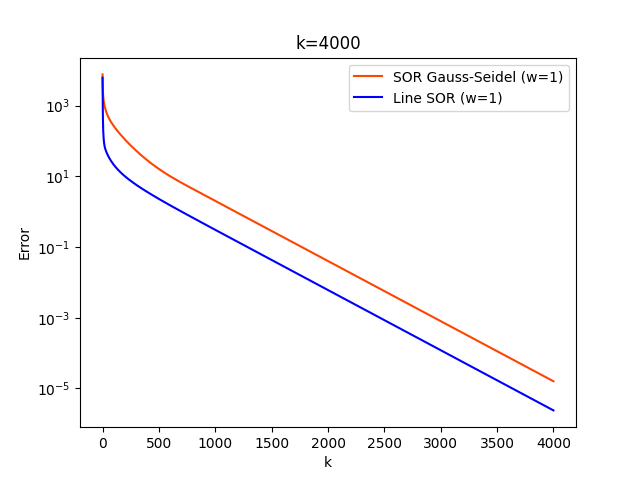
\includegraphics[width=0.7\textwidth]{LineVSpoint96gridpng.png}
    \label{LineVSpoint96gridpng.png}
    \caption{96x96 grid Comparsion}
\end{figure}



Compere to Point Gauss-Seidel method, Line SOR is much faster, and converge much faster:\\

For 4-cylinder platform, Line SOR could speed up to 48.35 it/s,
where Point GS-SOR iteraton speed is 21.73 it/s, or 563.64 VS. 141.83 CPU time,
that is almost twice faster as 
GS-SOR method. It also converge faster than point GS-SOR, 
for iteration calculation and need less iteration steps to converge to same level as 
GS-SOR.

\begin{figure}[H]
    \centering
    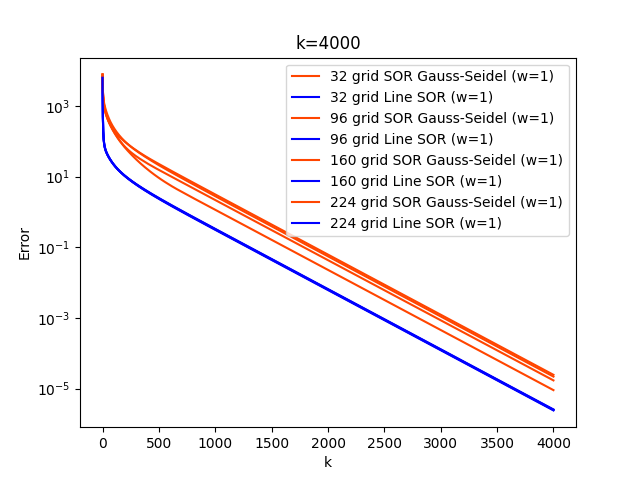
\includegraphics[width=0.7\textwidth]{LineVSpointTotal.png}
    \label{LineVSpointTotal.png}
    \caption{Different grid Comparsion}
\end{figure}

This plot compared Line SOR with point GS-SOR in different grid size, it could be shown
that Line SOR is converge much faster than point GS-SOR in each grid.










\section{(h) Potential Flow Calculate}



As we known, for potential flow, flow cannot pass the boundary into the cylinder, or 
anyother boundary not allowed flow to pass, we get:



\[
\frac{u_{\text{boundary}} - u_{\text{direction next point}}}{\Delta_{\text{direction}}} = 0
\]

\[
u_{\text{boundary}} = u_{\text{direction next point}}
\]


However, we need to create potential flow, which means it also need another boundary 
condition to allow flow pass by: 


\[
\frac{u_{\text{boundary}} - u_{\text{direction next point}}}{\Delta_{\text{direction}}} = Flow
\]

\[
u_{\text{boundary}} = u_{\text{direction next point}} + \Delta_{\text{direction}} Flow
\]


The boundary condition setting is shwoing below:

\begin{figure}[H]
    \centering
    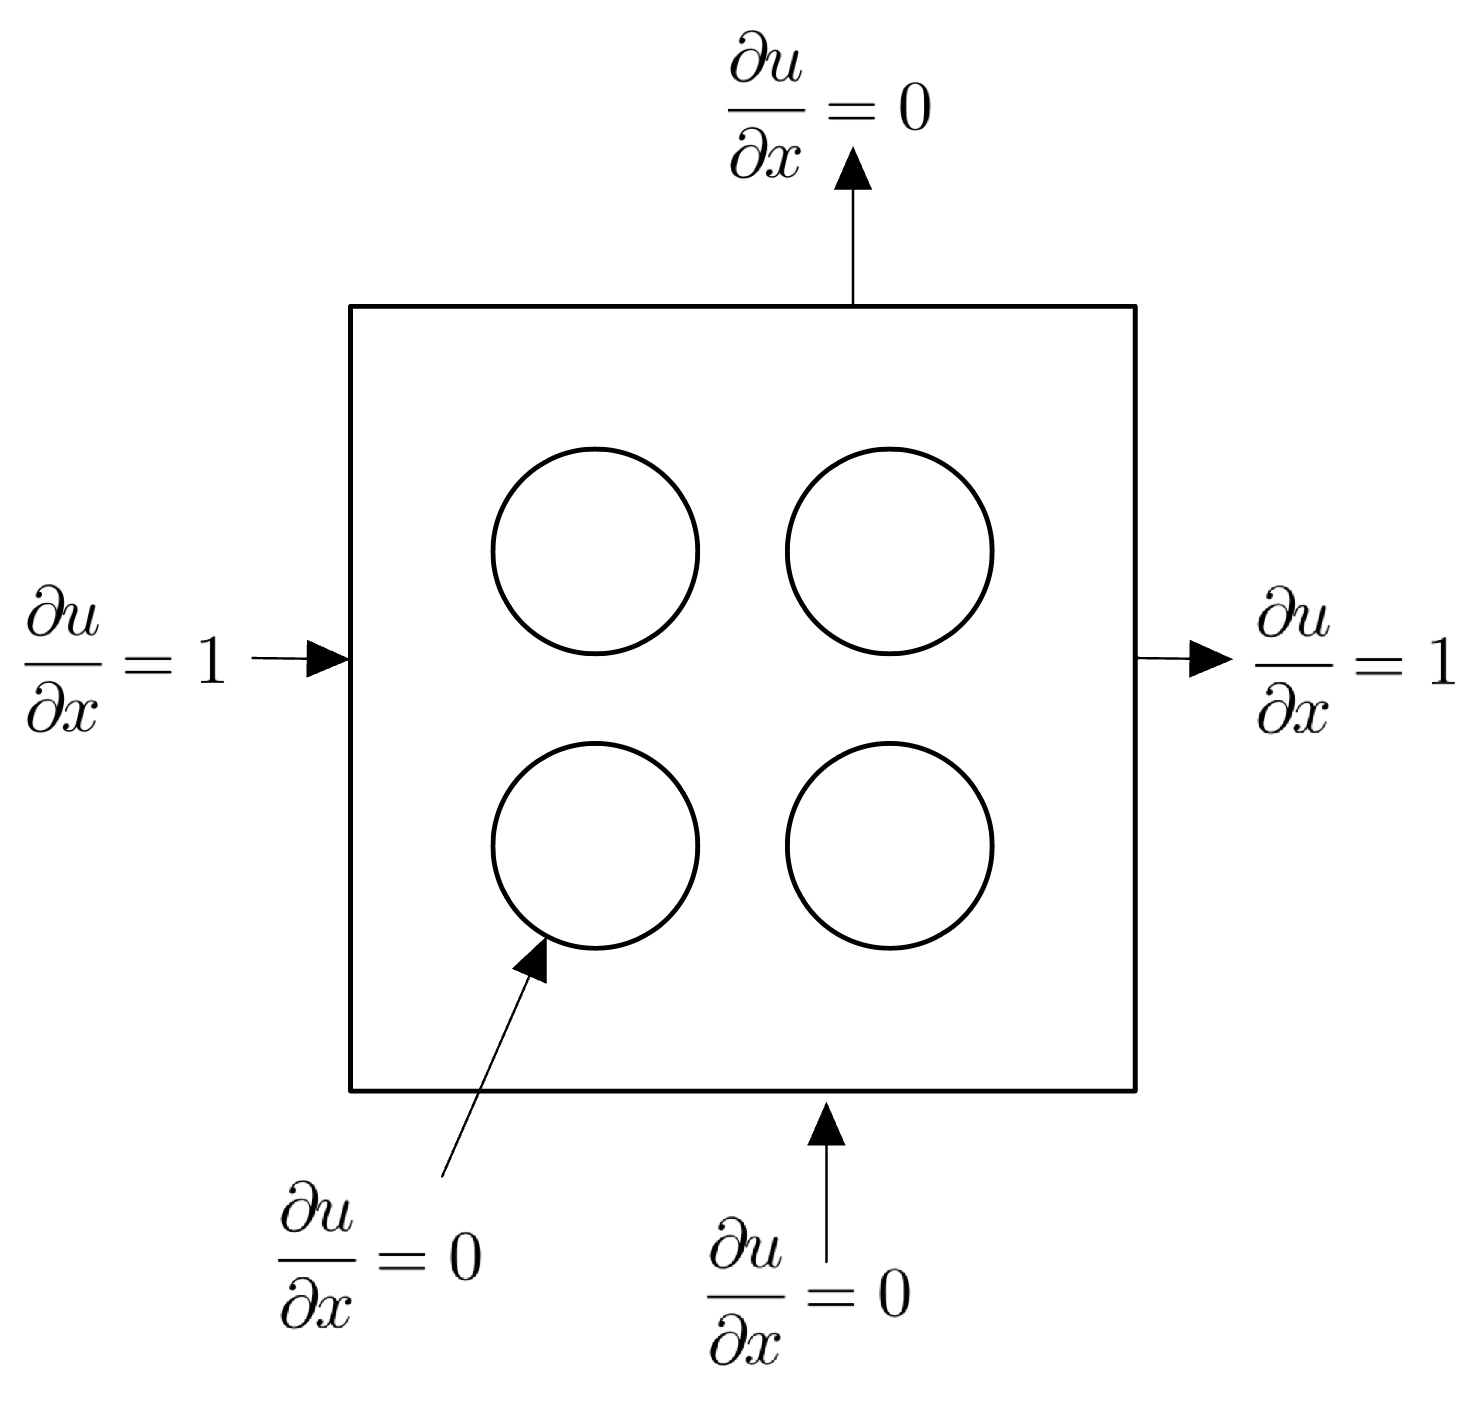
\includegraphics[width=0.5  \textwidth]{BoundaryVon.jpg}
    \label{BoundaryVon.jpg}
    \caption{Von-Neumann Boundary Condition}                                      
\end{figure}

We also need to expand our domain, the method is showing below:



\begin{figure}[H]
    \centering
    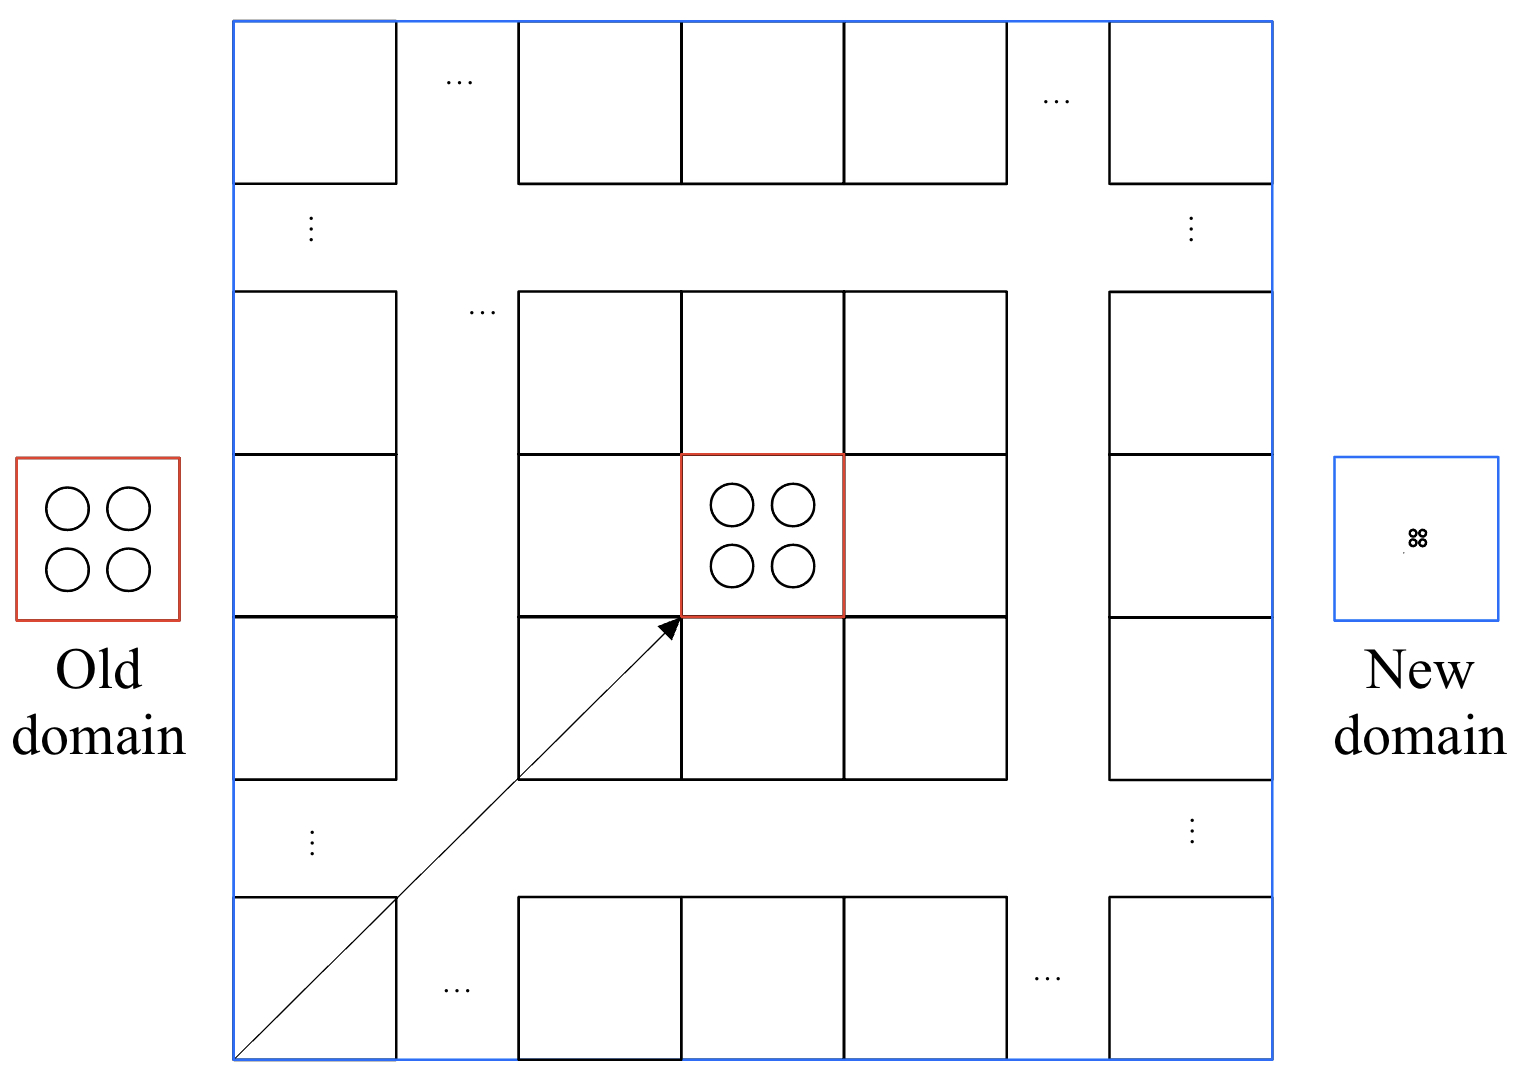
\includegraphics[width=0.7  \textwidth]{largedomain.jpg}
    \label{largedomain.jpg}
    \caption{Domain Change}                                      
\end{figure}

For this configuration, we only need to create a large domain, and transfer our 
inner boundary (4 cylinders) to that large domain, and calculate the result.








Apply this boundary condition, the result is showing below:



In the normal domain (not been expanded), the reuslt is showing below. 

\begin{figure}[H]
    \centering
    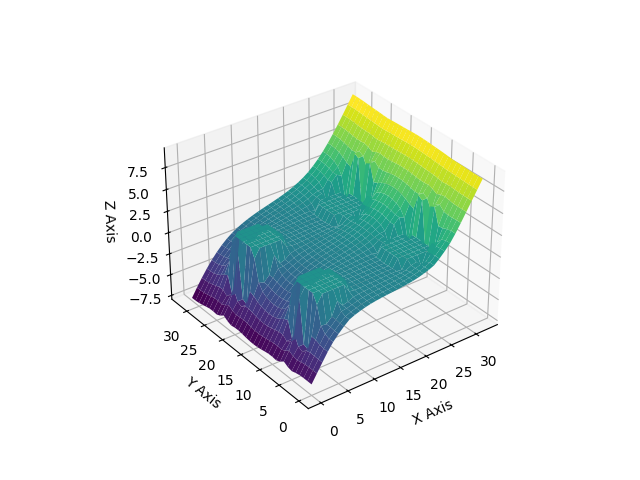
\includegraphics[width=0.7  \textwidth]{LargePotential001.png}
    \label{LargePotential001.png}
    \caption{Potential flow pass cylinder in domain}                                                                                                                                                                                                                                                                                                                                                                                                                                                                                                                                                                                                                                                                                                                                                                                                                                                                                                                                                                                                                                                                                                                                                                                                                                                                                                                                                                                                                                                                                                                                                                                                                                                                                                                                                                                                                                                                                                                                                                                                                                                                                                                                                                                                                                                                                                                                                                                                                                                                                                                                                                                                                                                                                                                                                                                                                                                                                                                                                                                                                                                                                                                                                                                                                                                                                                                                                                                                                                                                                                                                                                                                                                                                                                                                                                                                                                                                                                                                                                                                                                                                                                                                                                                                                                                                                                                                                                                                                                                                                                                                                                                                                                                                                                                                                                                                                                                                                                                                                         
\end{figure}

Expand the boundary to 9 times large, the result is showing below:


\begin{figure}[H]
    \centering
    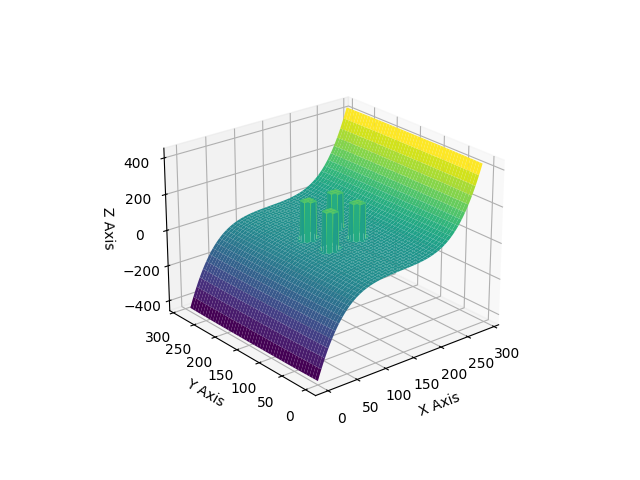
\includegraphics[width=0.7  \textwidth]{Large_Domain3d.png}
    \label{Large_Domain3d.png}
    \caption{Potential flow pass cylinder in domain on expanded Boundary}                                                                                                                                                                                                                                                                                                                                                                                                                                                                                                                                                                                                                                                                                                                                                                                                                                                                                                                                                                                                                                                                                                                                                                                                                                                                                                                                                                                                                                                                                                                                                                                                                                                                                                                                                                                                                                                                                                                                                                                                                                                                                                                                                                                                                                                                                                                                                                                                                                                                                                                                                                                                                                                                                                                                                                                                                                                                                                                                                                                                                                                                                                                                                                                                                                                                                                                                                                                                                                                                                                                                                                                                                                                                                                                                                                                                                                                                                                                                                                                                                                                                                                                                                                                                                                                                                                                                                                                                                                                                                                                                                                                                                                                                                                                                                                                                                                                                                                                                                         
\end{figure}




Calculate the pressure distribution and streamlines, the result is showing below:

\begin{figure}[H]
    \centering
    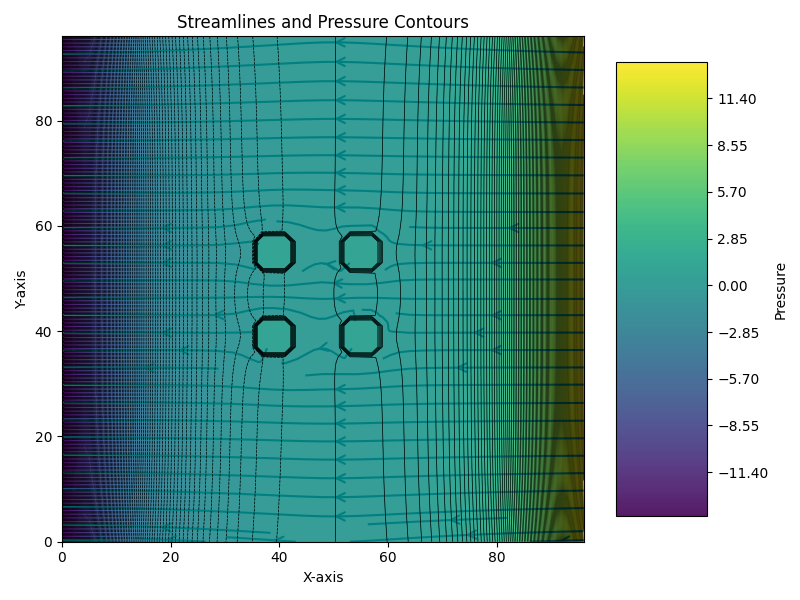
\includegraphics[width=0.6  \textwidth]{SteamPressureN=3.png}
    \label{SteamPressureN=3.png}
    \caption{Potential flow pass                                                                                                                                                                                                                                                                                                                                                                                                                                                                                                                                                                                                                                                                                                                                                                                                                                                                                                                                                                                                                                                                                                                                                                                                                                                                                                                                                                                                                                                                                                                                                                                                                                                                                                                                                                                                                                                                                                                                                                                                                                                                                                                                                                                                                                                                                                                                                                                                                                                                                                                                                                                                                                                                                                                                                                                                                                                                                                                                                                                                                                                                                                                                                                                                                                                                                                                                                                                                                                                                                                                                                                                                                                                                                                                                                                                                                                                                                                                                                                                                                                                                                                                                                                                                                                                                                                                                                                                                                                                                                                                                                                                                                                                                                                                                                                                                                                                                                                                                                               cylinder at large domain}
\end{figure}


For much large domain, the result is showing below:


\begin{figure}[H]
    \centering
    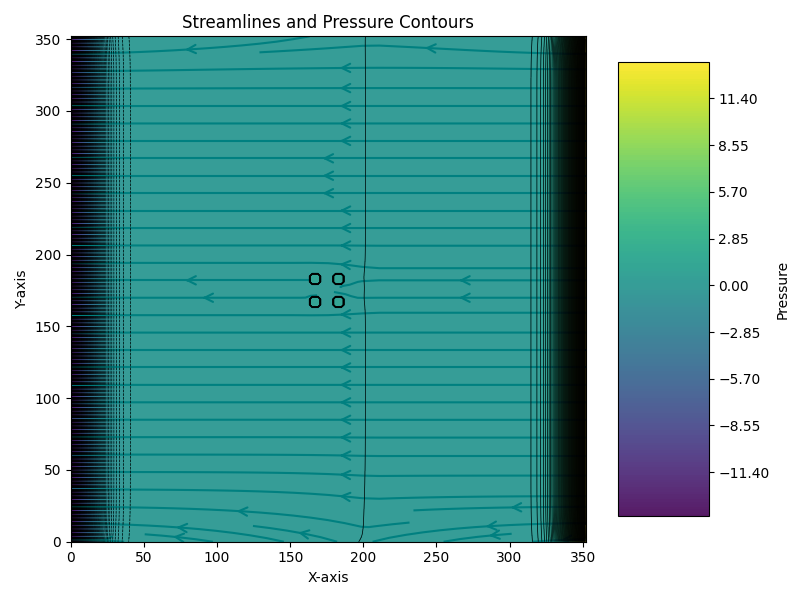
\includegraphics[width=0.6  \textwidth]{NlargeSteamPressure.png}
    \label{NlargeSteamPressure.png}
    \caption{Potential flow pass cylinders in large domain                                                                                                                                                                                                                                                                                                                                                                                                                                                                                                                                                                                                                                                                                                                                                                                                                                                                                                                                                                                                                                                                                                                                                                                                                                                                                                                                                                                                                                                                                                                                                                                                                                                                                                                                                                                                                                                                                                                                                                                                                                                                                                                                                                                                                                                                                                                                                                                                                                                                                                                                                                                                                                                                                                                                                                                                                                                                                                                                                                                                                                                                                                                                                                                                                                                                                                                                                                                                                                                                                                                                                                                                                                                                                                                                                                                                                                                                                                                                                                                                                                                                                                                                                                                                                                                                                                                                                                                                                                                                                                                                                                                                                                                                                                                                                                                                                                                                                                                                                           cylinder at large domain}
\end{figure}









%%%%%%%%%%%%%%%%%%%%%%%%%%%%%%%%%%%%%%%%%%%%%%%%%%%%%%%%%%%%%%%
%%%%%%%%%%%%%%%%%%%%%%%%%%%%%%%%%%%%%%%%%%%%%%%%%%%%%%%%%%%%%%%
%%%%%%%%%%%%%%%%%%%%%%%%%%%%%%%%%%%%%%%%%%%%%%%%%%%%%%%%%%%%%%%
\newpage
\section*{Appendix}

% 在目录中添加Appendix
\addcontentsline{toc}{section}{Appendix}



\begin{scriptsize}
    \begin{lstlisting}[language=python,caption={Python code--Functions for Grid Generator}]
    
        import copy 
        import matplotlib.pyplot as plt
        #import numpy as np
        import matplotlib as mpl
        
        
        import tqdm
        from tqdm import tqdm
        
        
        
        
        
        
        ##########################################################################################
        
        def real_True(number): # turn complex number to negative
            if isinstance(number, int):
                return number
            elif isinstance(number, float):
                return number
            elif isinstance(number, complex):
                return -100
        
            
        def int_True(number): # return int
            if isinstance(number, complex):
                return 0
            elif (number % 1==0):
                return -1
            else:
                return 0
            
        
        
        def IBcboundary(i, j ,  x_len, y_len, d, r): # calculate boundary points for \
        each i,j
            
            x = i * d
            y = j * d
            i_B1a_0= (x_len/2 - ( (r**2) - (y-y_len/2)**2 )**(1/2))/d
            i_B2b_0=(x_len/2 + ( (r**2) - (y-y_len/2)**2 )**(1/2))/d
            j_B1a_0=(y_len/2 - ( (r**2) - (x-x_len/2)**2 )**(1/2))/d
            j_B2b_0=(y_len/2 + ( (r**2) - (x-x_len/2)**2 )**(1/2))/d
        
        
            i_B1a= int(real_True(i_B1a_0)) 
            i_B2b=int(real_True(i_B2b_0)) +1 + int_True(i_B2b_0)
            j_B1a=int(real_True(j_B1a_0))
            j_B2b=int(real_True(j_B2b_0))+1 + int_True(j_B2b_0)
        
        
        
            return i_B1a, i_B2b, j_B1a, j_B2b
        ##########################################################################################
        
        
        
        
        ##########################################################################################
        
        def IBcondiitionor(  i_B1a, i_B2b, j_B1a, j_B2b, j_max, i_max): # use each \
        EP i,j to classify each EP
            GeneralP = [[0 for _ in range(0,j_max+1)] for _ in range(0,i_max+1)]
            P_xbl0 = copy.deepcopy(GeneralP)
            P_xbh0 = copy.deepcopy(GeneralP)
            P_ybl0 = copy.deepcopy(GeneralP)
            P_ybh0 = copy.deepcopy(GeneralP)
        
        
            C_xbl = copy.deepcopy(GeneralP)
            C_xbh = copy.deepcopy(GeneralP)
            C_ybl = copy.deepcopy(GeneralP)
            C_ybh = copy.deepcopy(GeneralP)
        
            C_edge = copy.deepcopy(GeneralP)
        
            C_xlyl = copy.deepcopy(GeneralP)
            C_xlyh = copy.deepcopy(GeneralP)
            C_xhyl = copy.deepcopy(GeneralP)
            C_xhyh = copy.deepcopy(GeneralP)
        
            
        
            a = 1
            b = 10
            c = 41
            d = 51
        
        
            for j in range(1,j_max):
                if i_B1a[j]>0:
                    P_xbl0[j][i_B1a[j]] = a
                if i_B2b[j]>0:
                    P_xbh0[j][i_B2b[j]] = b
            for i in range(1,i_max):
                if j_B1a[i]>0:
                    P_ybl0[j_B1a[i]][i] = c
                if j_B2b[i]>0:
                    P_ybh0[j_B2b[i]][i] = d
        
            for j in range(1,j_max):
                for i in range(1,i_max):
                    if ((P_xbl0[j][i] + P_xbh0[j][i]==a+b) or (P_ybl0[j][i] + P_ybh0[j][i]\
                    ==c+d)): # find out grid point just on the edge -->C_edge
                        C_edge[j][i] = 1  
        
                    if (P_xbl0[j][i] + P_ybl0[j][i] == a+c):    
                     # find out where the edge cut x and y line, where x low y low -->C_xlyl
                        C_xlyl[j][i] = 1 - C_edge[j][i]
                    if (P_xbl0[j][i] + P_ybh0[j][i] == a+d):   
                    # find out where the edge cut x and y line, where x low y high -->C_xlyh
                        C_xlyh[j][i] = 1 - C_edge[j][i]
                    if (P_xbh0[j][i] + P_ybl0[j][i] == b+c):   
                    # find out where the edge cut x and y line, where x high y low -->C_xhyl
                        C_xhyl[j][i] = 1 - C_edge[j][i]
                    if (P_xbh0[j][i] + P_ybh0[j][i] == b+d):   
                    # find out where the edge cut x and y line, where x high y high -->C_xhyh
                        C_xhyh[j][i] = 1 - C_edge[j][i]
                    
                    special = C_edge[j][i] +  C_xlyl[j][i] + C_xlyh[j][i] + C_xhyl[j][i]\
                      + C_xhyh[j][i]
                
            for j in range(1,j_max):
                for i in range(1,int(i_max/2)):
        
                    C_xbl[j][i] = P_xbl0[j][i]//a - C_edge[j][i] -  C_xlyl[j][i] - \
                    C_xlyh[j][i] # find out where edge ONLY cut x low lines 
            
            for j in range(1,j_max):
                for i in range(int(i_max/2),i_max):
        
                    C_xbh[j][i] = P_xbh0[j][i]//b - C_edge[j][i]  - C_xhyl[j][i] - \
                    C_xhyh[j][i] # find out where edge ONLY cut x high lines 
        
            for j in range(1,int(j_max/2)):
                for i in range(1,i_max):
                    C_ybl[j][i] = P_ybl0[j][i]//c - C_edge[j][i] - C_xlyl[j][i]  - \
                    C_xhyl[j][i] # find out where edge ONLY cut y low lines
        
            for j in range(int(j_max/2),j_max):
                for i in range(1,i_max):
                    C_ybh[j][i] = P_ybh0[j][i]//d - C_edge[j][i]  - C_xlyh[j][i]  - \
                    C_xhyh[j][i] # find out where edge ONLY cut y high lines 
        
            
        
            return C_xbl, C_xbh, C_ybl, C_ybh, C_edge, C_xlyl, C_xlyh, C_xhyl, C_xhyh
        ##########################################################################################
        
        
        
        
        
        
        
        
        ##########################################################################################
        def Cinner_and_IBi(i_max, j_max, i_Bmin, i_Bmax, j_Bmin, j_Bmax, C_xbl, C_xbh, \
        C_ybl, C_ybh, C_edge, C_xlyl, C_xlyh, C_xhyl, C_xhyh):
        
            C_total = copy.deepcopy(C_xbl)
            C_inner = copy.deepcopy(C_xbl)
        
            for j in range(0,j_Bmax+1):
                for i in range(0,i_Bmax+1):
                    C_total[j][i] = C_xbl[j][i] + C_xbh[j][i] + C_ybl[j][i] + \
                    C_ybh[j][i] + C_edge[j][i] + C_xlyl[j][i] + C_xlyh[j][i] + \
                    C_xhyl[j][i] + C_xhyh[j][i]
                    C_inner[j][i] = 1 - C_total[j][i]
        
            i_l = [0 for _ in range(0, j_max+1)]
            i_h = [0 for _ in range(0, j_max+1)]
        
        
        
            for j in range(0,j_Bmin):
                for i in range(0,i_max):
                    C_inner[j][i] = 0
        
            for j in range(j_Bmax+1,j_max):
                for i in range(0,i_max):
                    C_inner[j][i] = 0
        
            
            for j in range(j_Bmin,j_Bmax+1):
                for i in range(0,i_max+1):
                    if C_total[j][i] == 1:
                        i_l[j] = i
                        break
                    else: C_inner[j][i] -= 1
                for i in range(i_max,i_Bmin,-1):
                    if C_total[j][i] == 1:
                        i_h[j] = i
                        break
                    else: C_inner[j][i] -= 1
        
            for j in range(0,j_max+1):
                for i in range(0,i_max+1):
                    if C_inner[j][i] < 0: C_inner[j][i] = 0
            
            return C_inner, C_total, i_l, i_h # C_total means the total inner \
            boundary, while C_inner is the points in the inner boundary
        ##########################################################################################
        
        
        
    \end{lstlisting}
\end{scriptsize}





\begin{scriptsize}
    \begin{lstlisting}[language=python,caption={Python code-Functions for iteration Calculator}]
    
        ##########################################################################################
        def calculator_GSSOR(P_inputSOR, j_limlow, j_limhigh, i_limlow, i_limhigh , w): 
        #Gauss Sadiel SOR method Pin-->Pout
            PgSOR = copy.deepcopy(P_inputSOR)
            for j in range(j_limlow, j_limhigh+1):
                for i in range(i_limlow, i_limhigh+1): 
                    PgSOR[j][i] = \
                        1/4 * (  PgSOR[j][i-1] + P_inputSOR[j][i+1] + PgSOR[j-1][i] \
                        + P_inputSOR[j+1][i] )*w + (1-w)*P_inputSOR[j][i]
            return PgSOR
        
        
        
        
        def Point_Calculator_IBGSSOR(P, PgSOR, j, i, w, C_inner, C_total, C_xbl, C_xbh, \
        C_ybl, C_ybh, C_edge, C_xlyl, C_xlyh, C_xhyl, C_xhyh):
            
        
            PgSOR[j][i] = \
                (1/4 * (  PgSOR[j][i-1] + P[j][i+1] + PgSOR[j-1][i] + P[j+1][i] )*w + \
                (1-w)*P[j][i])*(1-C_total[j][i])*(1-C_inner[j][i]) +(\
                    C_edge[j][i] \
                + C_xbl[j][i] * IB1_cal(PgSOR[j][i-1],PgSOR[j-1][i],P[j+1][i])\
                + C_xbh[j][i] * IB1_cal(P[j][i+1],PgSOR[j-1][i],P[j+1][i])\
                + C_ybl[j][i] * IB1_cal(PgSOR[j-1][i],PgSOR[j][i-1],P[j][i+1])\
                + C_ybh[j][i] * IB1_cal(P[j+1][i],PgSOR[j][i-1],P[j][i+1])\
                + C_xlyl[j][i] * IB2_cal(PgSOR[j][i-1],PgSOR[j-1][i])\
                + C_xlyh[j][i] * IB2_cal(PgSOR[j][i-1],P[j+1][i])\
                + C_xhyl[j][i] * IB2_cal(P[j][i+1],PgSOR[j-1][i])\
                + C_xhyh[j][i] * IB2_cal(P[j][i+1],P[j+1][i]) ) *(1-C_inner[j][i])\
                + C_inner[j][i] * 1
            
            return PgSOR[j][i]
        ##########################################################################################
        
        ##########################################################################################
        def IB1_cal(a,b,c):
            P = (a*4/3+8/3+b+c)/6
            return P
        ##########################################################################################
        
        ##########################################################################################
        def IB2_cal(a,b):
            P = (a+b)/6 + 2/3
            return P
        ##########################################################################################
            

        
        
        
        ##########################################################################################
        def GSSOR_Solver(P_input, i_max, j_max, i_Bmin, i_Bmax, j_Bmin, j_Bmax, i_l, i_h, w \
                         ,C_inner, C_total, C_xbl, C_xbh, C_ybl, C_ybh, C_edge, C_xlyl, \
                         C_xlyh, C_xhyl, C_xhyh):
        
            # Solve for low GP
            P = copy.deepcopy(P_input)
            
            P = calculator_GSSOR(P, 1 , j_Bmin-1, 1 , i_max-1 , w)
        
            # Solve for EP + GP in middle
            PgSOR = copy.deepcopy(P)
            for j in range(j_Bmin, j_Bmax+1):
        
        
                # solve for left GP
                for i in range(1, i_l[j]): 
                    PgSOR[j][i] = \
                        1/4 * (  PgSOR[j][i-1] + P[j][i+1] + PgSOR[j-1][i] + P[j+1][i] )\
                        *w + (1-w)*P[j][i]
                P = PgSOR
        
        
                # solve for middle (including point judgement (mathematically))
                for i in range(i_l[j], i_h[j]+1):
                    PgSOR[j][i] = Point_Calculator_IBGSSOR(P, PgSOR, j, i, w,\
                                                       C_inner, C_total, C_xbl, C_xbh, \
                                                       C_ybl, C_ybh, C_edge, C_xlyl, \
                                                       C_xlyh, C_xhyl, C_xhyh)
                P = PgSOR
                    
                # solve for right GP
                for i in range(i_h[j]+1, i_max):
                    PgSOR[j][i] = \
                        1/4 * (  PgSOR[j][i-1] + P[j][i+1] + PgSOR[j-1][i] + P[j+1][i] )\
                        *w + (1-w)*P[j][i]
                P = PgSOR
            
            # solve for high GP
            P = calculator_GSSOR(P, j_Bmax+1 , j_max-1 ,1, i_max-1 , w)
        
            return P
            
        ##########################################################################################
        
        
    \end{lstlisting}
\end{scriptsize}



\begin{scriptsize}
    \begin{lstlisting}[language=python,caption={Python code-Functions for Iteration Solver and Result Analysist}]
    
        ##########################################################################################
        
        
        
        def Res(r,Pin,d,i_l,i_h,i_max,j_max): #calcuate residual (Pin, source)-->Rout
            P = copy.deepcopy(Pin)
            rc = copy.deepcopy(r)
            for j in range(1,j_max):
                for i in range(1,i_l[j]): 
                    rc[j][i] = \
                        ( P[j][i-1] + P[j][i+1] + P[j-1][i] + P[j+1][i] - 4*P[j][i] ) 
                for i in range(i_h[j]+1,i_max): 
                    rc[j][i] = \
                        ( P[j][i-1] + P[j][i+1] + P[j-1][i] + P[j+1][i] - 4*P[j][i] ) 
            return rc
        
        def Error(r_in, i_max, j_max): #calculate error Rin-->e out
            r = copy.deepcopy(r_in)
            e = 0
            for j in range(1,j_max):
                for i in range(1,i_max): 
                    e += abs(r[j][i])   #**2
            return e
        
        
        
        
        
        
        def Generaleach(x_len,y_len,d,r,x_c,y_c, Kmax, w):
            ######### create grid information
            i_max = int(x_len/d)  # i in [0,i_max]
            j_max = int(y_len/d)
        
        
            P = [[0 for _ in range(0,j_max+1)] for _ in range(0,i_max+1)]
        
            import random
            for j in range(1,y_len-1):
                for i in range(1,x_len-1):
                    P[j][i] = random.randint(-1,1)
        
        
        
        
            ######### define inner boundary limit
            i_Bmin = int((x_c-r)/d)
            i_Bmax = int((x_c+r)/d) +1 +  int_True((x_c+r)/d)
            j_Bmin = int((y_c-r)/d)
            j_Bmax = int((y_c+r)/d) +1 +  int_True((y_c+r)/d)
        
        
            ######### define inner boundary
            iline = [0 for _ in range(0,i_max+1)]
            jline = [0 for _ in range(0,j_max+1)]
        
            i_B1a = copy.deepcopy(iline)
            i_B2b = copy.deepcopy(iline)
            j_B1a = copy.deepcopy(jline)
            j_B2b = copy.deepcopy(jline)
        
        
        
            for j in range(j_Bmin,j_Bmax+1):
                for i in range(i_Bmin, i_Bmax+1):
                    i_B1a[j], i_B2b[j], j_B1a[i], j_B2b[i] = IBcboundary(i, j ,  \
                    x_len, y_len, d, r)
        
        
            C_xbl, C_xbh, C_ybl, C_ybh, C_edge, C_xlyl, C_xlyh, C_xhyl, C_xhyh \
            = IBcondiitionor(  i_B1a, i_B2b, j_B1a, j_B2b, j_max, i_max)
        
            C_inner, C_total, i_l, i_h = Cinner_and_IBi(i_max, j_max, \
            i_Bmin, i_Bmax, j_Bmin, j_Bmax, \
             C_xbl, C_xbh, C_ybl, C_ybh, C_edge, C_xlyl, C_xlyh, C_xhyl, C_xhyh)     
        
        
        
        
            ##################################################### Iteration Part ###################################################################################
        
        
        
            r1 = copy.deepcopy(P)
            e1 = [0 for _ in range(0,Kmax+1)]
        
        
        
            P_input = copy.deepcopy(P)
            
        
            for k in tqdm(range(0,Kmax+1)):
        
                P = GSSOR_Solver(P_input, i_max, j_max, i_Bmin, i_Bmax, \
                j_Bmin, j_Bmax, i_l, i_h, w , \
                         C_inner, C_total, C_xbl, C_xbh, C_ybl, C_ybh, C_edge, \
                         C_xlyl, C_xlyh, C_xhyl, C_xhyh)
                P_input = copy.deepcopy(P)
        
                r1 = Res(r1,P,d,i_l,i_h,i_max,j_max)
                e1[k] = Error(r1, i_max, j_max)
        
            return e1
                
        
        
        ############
        
        
        def eploting(   e32, e96, e160, e224,    d,    Kmax     ):
            x = [0 for _ in range(0, Kmax+1)]
            for c in range(0,Kmax+1):
                x[c] = c
            plt.plot(x, e32, color = 'red', label = 'Grid Size 32')
            plt.plot(x, e96, color = 'orange', label = 'Grid Size 96')
            plt.plot(x, e160, color = 'blue', label = 'Grid Size 160')
            plt.plot(x, e224, color = 'green', label = 'Grid Size 224')
            plt.legend()
        
            plt.yscale('log')
            plt.xlabel('k')
            plt.ylabel('Error')
            #plt.ylim(0,1)
            plt.ylim(10**(-6),1)
        
            plt.title("Kmax=%d"%Kmax)
        
        
        
        
        
            plt.show()
        
        
        
        
        def Ploting3D(P):
            import matplotlib.pyplot as plt
            from mpl_toolkits.mplot3d import Axes3D
            import numpy as np
        
            data = P
        
        
            data_np = np.array(data)
        
            rows, cols = len(data), len(data[0])
        
            x = np.linspace(0, cols - 1, cols)
            y = np.linspace(0, rows - 1, rows)
            x, y = np.meshgrid(x, y)
        
            fig = plt.figure()
            ax = fig.add_subplot(111, projection='3d')
        
            ax.plot_surface(x, y, data_np, cmap='viridis')
        
            ax.set_xlabel('X Axis')
            ax.set_ylabel('Y Axis')
            ax.set_zlabel('Z Axis')
        
            plt.show()
        
        
         
                
        
    \end{lstlisting}
    \end{scriptsize}
    
    
    
    
    
    
    
    
    

\begin{scriptsize}
\begin{lstlisting}[language=python,caption={The python Source code of Main Function}]

    
    def main():
    
        ########## input mathematical domain inforamtion
        x_len = y_len = len = 1
        r = 0.25
        x_c = x_len/2
        y_c = y_len/2
    
    
        ########### Iteration Setup
    
        w =1
        Kmax = 10000
    
    
        
    
        #print(P)
        #Ploting3D(P)
    
        ######### input numerical grid information
        size = 32
    
        d = len/size
    
    
        e32 = Generaleach(x_len,y_len,d,r,x_c,y_c, Kmax, w)
    
        ######### input numerical grid information
        size = 96
    
        d = len/size
    
    
        e96 = Generaleach(x_len,y_len,d,r,x_c,y_c, Kmax, w)
    
        ######### input numerical grid information
        size = 160
    
        d = len/size
    
    
        e160 = Generaleach(x_len,y_len,d,r,x_c,y_c, Kmax, w)
    
        ######### input numerical grid information
        size = 224
    
        d = len/size
    
    
        e224 = Generaleach(x_len,y_len,d,r,x_c,y_c, Kmax, w)
    
    
        eploting(   e32, e96, e160, e224,    d,    Kmax     )
        
    
    
    
    if __name__ == "__main__":
        main()
    


    
\end{lstlisting}
\end{scriptsize}





\begin{scriptsize}
    \begin{lstlisting}[language=python,caption={Python code-Potential Flow}]
        import copy 
        import matplotlib.pyplot as plt
        import numpy as np
        import matplotlib as mpl
        
        
        import tqdm
        from tqdm import tqdm
        
        
        
        ######################## TEST FUNCTION
        
        
        
        
        
        
        
        
        
        
        
        
        ##########################################################################################
        
        def real_True(number): # turn complex number to negative
            if isinstance(number, int):
                return number
            elif isinstance(number, float):
                return number
            elif isinstance(number, complex):
                return -100
        
            
        def int_True(number): # return int
            if isinstance(number, complex):
                return 0
            elif (number % 1==0):
                return -1
            else:
                return 0
            
        
        
        def IBcboundary(i, j ,  x_len, y_len, d, r): 
        # calculate boundary points for each i,j
            
            x = i * d
            y = j * d
            i_B1a_0= (x_len/2 - ( (r**2) - (y-y_len/2)**2 )**(1/2))/d
            i_B2b_0=(x_len/2 + ( (r**2) - (y-y_len/2)**2 )**(1/2))/d
            j_B1a_0=(y_len/2 - ( (r**2) - (x-x_len/2)**2 )**(1/2))/d
            j_B2b_0=(y_len/2 + ( (r**2) - (x-x_len/2)**2 )**(1/2))/d
        
        
            i_B1a= int(real_True(i_B1a_0)) 
            i_B2b=int(real_True(i_B2b_0)) +1 + int_True(i_B2b_0)
            j_B1a=int(real_True(j_B1a_0))
            j_B2b=int(real_True(j_B2b_0))+1 + int_True(j_B2b_0)
        
        
        
            return i_B1a, i_B2b, j_B1a, j_B2b
        ##########################################################################################
        
        
        
        
        ##########################################################################################
        
        def IBcondiitionor(  i_B1a, i_B2b, j_B1a, j_B2b, j_max, i_max): 
        # use each EP i,j to classify each EP
            GeneralP = [[0 for _ in range(0,j_max+1)] for _ in range(0,i_max+1)]
            P_xbl0 = copy.deepcopy(GeneralP)
            P_xbh0 = copy.deepcopy(GeneralP)
            P_ybl0 = copy.deepcopy(GeneralP)
            P_ybh0 = copy.deepcopy(GeneralP)
        
        
            C_xbl = copy.deepcopy(GeneralP)
            C_xbh = copy.deepcopy(GeneralP)
            C_ybl = copy.deepcopy(GeneralP)
            C_ybh = copy.deepcopy(GeneralP)
        
            C_edge = copy.deepcopy(GeneralP)
        
            C_xlyl = copy.deepcopy(GeneralP)
            C_xlyh = copy.deepcopy(GeneralP)
            C_xhyl = copy.deepcopy(GeneralP)
            C_xhyh = copy.deepcopy(GeneralP)
        
            
        
            a = 1
            b = 10
            c = 41
            d = 51
        
        
            for j in range(1,j_max):
                if i_B1a[j]>0:
                    P_xbl0[j][i_B1a[j]] = a
                if i_B2b[j]>0:
                    P_xbh0[j][i_B2b[j]] = b
            for i in range(1,i_max):
                if j_B1a[i]>0:
                    P_ybl0[j_B1a[i]][i] = c
                if j_B2b[i]>0:
                    P_ybh0[j_B2b[i]][i] = d
        
            for j in range(1,j_max):
                for i in range(1,i_max):
                    if ((P_xbl0[j][i] + P_xbh0[j][i]==a+b) or (P_ybl0[j][i] + P_ybh0[j][i]==c+d)): 
                    # find out grid point just on the edge -->C_edge
                        C_edge[j][i] = 1  
        
                    if (P_xbl0[j][i] + P_ybl0[j][i] == a+c):     
                    # find out where the edge cut x and y line, where x low y low -->C_xlyl
                        C_xlyl[j][i] = 1 - C_edge[j][i]
                    if (P_xbl0[j][i] + P_ybh0[j][i] == a+d):   
                    # find out where the edge cut x and y line, where x low y high -->C_xlyh
                        C_xlyh[j][i] = 1 - C_edge[j][i]
                    if (P_xbh0[j][i] + P_ybl0[j][i] == b+c):   
                    # find out where the edge cut x and y line, where x high y low -->C_xhyl
                        C_xhyl[j][i] = 1 - C_edge[j][i]
                    if (P_xbh0[j][i] + P_ybh0[j][i] == b+d):   
                    # find out where the edge cut x and y line, where x high y high -->C_xhyh
                        C_xhyh[j][i] = 1 - C_edge[j][i]
                    
                    special = C_edge[j][i] +  C_xlyl[j][i] + C_xlyh[j][i] + C_xhyl[j][i]  + C_xhyh[j][i]
                
            for j in range(1,j_max):
                for i in range(1,int(i_max/2)):
        
                    C_xbl[j][i] = P_xbl0[j][i]//a - C_edge[j][i] -  C_xlyl[j][i] - C_xlyh[j][i] 
                    # find out where edge ONLY cut x low lines 
            
            for j in range(1,j_max):
                for i in range(int(i_max/2),i_max):
        
                    C_xbh[j][i] = P_xbh0[j][i]//b - C_edge[j][i]  - C_xhyl[j][i] - C_xhyh[j][i] 
                    # find out where edge ONLY cut x high lines 
        
            for j in range(1,int(j_max/2)):
                for i in range(1,i_max):
                    C_ybl[j][i] = P_ybl0[j][i]//c - C_edge[j][i] - C_xlyl[j][i]  - C_xhyl[j][i] 
                    # find out where edge ONLY cut y low lines
        
            for j in range(int(j_max/2),j_max):
                for i in range(1,i_max):
                    C_ybh[j][i] = P_ybh0[j][i]//d - C_edge[j][i]  - C_xlyh[j][i]  - C_xhyh[j][i] 
                    # find out where edge ONLY cut y high lines 
        
            
        
            return C_xbl, C_xbh, C_ybl, C_ybh, C_edge, C_xlyl, C_xlyh, C_xhyl, C_xhyh
        ##########################################################################################
        
        
        
        
        ##########################################################################################
        def Cinner_and_IBi(i_max, j_max, i_Bmin, i_Bmax, j_Bmin, j_Bmax, C_xbl, C_xbh, C_ybl, C_ybh,\ 
         C_edge, C_xlyl, C_xlyh, C_xhyl, C_xhyh):
        
            C_total = copy.deepcopy(C_xbl)
            C_inner = copy.deepcopy(C_xbl)
        
            for j in range(0,j_Bmax+1):
                for i in range(0,i_Bmax+1):
                    C_total[j][i] = C_xbl[j][i] + C_xbh[j][i] + C_ybl[j][i] + C_ybh[j][i]\ 
                     + C_edge[j][i] + C_xlyl[j][i] + C_xlyh[j][i] + C_xhyl[j][i] + C_xhyh[j][i]
                    C_inner[j][i] = 1 - C_total[j][i]
        
            i_l = [0 for _ in range(0, j_max+1)]
            i_h = [0 for _ in range(0, j_max+1)]
        
        
        
            for j in range(0,j_Bmin):
                for i in range(0,i_max):
                    C_inner[j][i] = 0
        
            for j in range(j_Bmax+1,j_max):
                for i in range(0,i_max):
                    C_inner[j][i] = 0
        
            
            for j in range(j_Bmin,j_Bmax+1):
                for i in range(0,i_max+1):
                    if C_total[j][i] == 1:
                        i_l[j] = i
                        break
                    else: C_inner[j][i] -= 1
                for i in range(i_max,i_Bmin,-1):
                    if C_total[j][i] == 1:
                        i_h[j] = i
                        break
                    else: C_inner[j][i] -= 1
        
            for j in range(0,j_max+1):
                for i in range(0,i_max+1):
                    if C_inner[j][i] < 0: C_inner[j][i] = 0
            
            return C_inner, C_total, i_l, i_h 
            # C_total means the total inner boundary, while C_inner is the points in the inner boundary
        ##########################################################################################
        
        
        
        def inner_boundary_generator(i_max, j_max, d, x_len, y_len, len, x_c, y_c, r, size):
        
            
        
            ######### define inner boundary limit
            i_Bmin = int((x_c-r)/d)
            i_Bmax = int((x_c+r)/d) +1 +  int_True((x_c+r)/d)
            j_Bmin = int((y_c-r)/d)
            j_Bmax = int((y_c+r)/d) +1 +  int_True((y_c+r)/d)
        
        
            ######### define inner boundary
            iline = [0 for _ in range(0,i_max+1)]
            jline = [0 for _ in range(0,j_max+1)]
        
            i_B1a = copy.deepcopy(iline)
            i_B2b = copy.deepcopy(iline)
            j_B1a = copy.deepcopy(jline)
            j_B2b = copy.deepcopy(jline)
        
        
        
            for j in range(j_Bmin,j_Bmax+1):
                for i in range(i_Bmin, i_Bmax+1):
                    i_B1a[j], i_B2b[j], j_B1a[i], j_B2b[i] = \ 
                    IBcboundary(i, j ,  x_len, y_len, d, r)
        
        
            C_xbl, C_xbh, C_ybl, C_ybh, C_edge, C_xlyl, C_xlyh, C_xhyl, C_xhyh = \ 
            IBcondiitionor(  i_B1a, i_B2b, j_B1a, j_B2b, j_max, i_max)
        
            C_inner, C_total, i_l, i_h = Cinner_and_IBi(i_max, j_max, i_Bmin, i_Bmax, j_Bmin, j_Bmax, \
                                                        C_xbl, C_xbh, C_ybl, C_ybh, C_edge, C_xlyl,\ 
                                                        C_xlyh, C_xhyl, C_xhyh)    
        
            return  C_inner, C_total, i_l, i_h,\
                 i_Bmin, i_Bmax, j_Bmin, j_Bmax,\
                    C_xbl, C_xbh, C_ybl, C_ybh, C_edge, C_xlyl, C_xlyh, C_xhyl, C_xhyh \
                    
        
        def multiplyA(P, C_in):
        
            C_out = copy.deepcopy(P)
        
            for j in range(1, len(C_in)-1):
                for i in range(1,len(C_in)-1):
                    C_out[j][i] += C_in[j][i]
                    C_out[j][i+len(C_in)-1] += C_in[j][i]
                    C_out[j+len(C_in)-1][i] += C_out[j][i]
                    C_out[j+len(C_in)-1][i+len(C_in)-1] = C_in[j][i]
            return C_out
        
        
        def OBdefine(P):
            i_max =len(P)
            j_max = len(P)
            C_Oxl = copy.deepcopy(P)
            C_Oxh = copy.deepcopy(P)
            C_Oyl = copy.deepcopy(P)
            C_Oyh = copy.deepcopy(P)
            for i in range(1,i_max):
                C_Oxl[0][i] = 1
                C_Oxh [j_max][i] = 1
            for j in range(0,j_max+1):
                C_Oyl [j][0] = 1
                C_Oyh [j][i_max] = 1
        
            return C_Oxl, C_Oxh, C_Oyl, C_Oyh
        
        
        
        def Large_transfer(F, n, j_max, i_max):
            large_j_max = n * j_max
            large_i_max = n * i_max
        
            center_j_large = large_j_max // 2
            center_i_large = large_i_max // 2
            
            center_j_small = j_max // 2
            center_i_small = i_max // 2
        
            start_j = center_j_large - center_j_small - (0 if j_max % 2 else 1)
            start_i = center_i_large - center_i_small - (0 if i_max % 2 else 1)
        
            P = [[0 for _ in range(large_i_max)] for _ in range(large_j_max)]
        
            for j in range(j_max):
                for i in range(i_max):
                    P[start_j + j][start_i + i] = F[j][i]
        
            return P
                
        
            
        
            
        ##########################################################################################
        def calculator_GSSOR(P_inputSOR, j_limlow, j_limhigh, i_limlow, i_limhigh , w): 
        #Gauss Sadiel SOR method Pin-->Pout
            PgSOR = copy.deepcopy(P_inputSOR)
            for j in range(j_limlow, j_limhigh+1):
                for i in range(i_limlow, i_limhigh+1): 
                    PgSOR[j][i] = \
                        1/4 * (  PgSOR[j][i-1] + P_inputSOR[j][i+1] + PgSOR[j-1][i] + \ 
                        P_inputSOR[j+1][i] )*w + (1-w)*P_inputSOR[j][i]
            return PgSOR
        
        
        
        
        def Point_Calculator_IBGSSOR(P, PgSOR, j, i, w, C_inner, C_total, C_xbl, C_xbh, \ 
        C_ybl, C_ybh, C_edge, C_xlyl, C_xlyh, C_xhyl, C_xhyh):
        
        
            PgSOR[j][i] = \
                (1/4 * (  PgSOR[j][i-1] + P[j][i+1] + PgSOR[j-1][i] + P[j+1][i] )*w \ 
                + (1-w)*P[j][i])*(1-C_total[j][i]-C_inner[j][i]) \
                + C_xbl[j][i] * PgSOR[j][i-1]\
                + C_xbh[j][i] * P[j][i+1]\
                + C_ybl[j][i] * PgSOR[j-1][i]\
                + C_ybh[j][i] * P[j+1][i]\
                + C_inner[j][i] *200\
                + C_xlyl[j][i] * (P[j-1][i]+P[j][i-1])/2\
                + C_xlyh[j][i] * (P[j][i-1]+P[j+1][i])/2\
                + C_xhyl[j][i] * (P[j][i+1]+P[j-1][i])/2\
                + C_xhyh[j][i] * (P[j+1][i]+P[j][i+1])/2\
                
            
            return PgSOR[j][i]
        ##########################################################################################
        
        ##########################################################################################
        def IB1_cal(a,b,c):
            P = (a*4/3+8/3+b+c)/6
            return P
        ##########################################################################################
        
        ##########################################################################################
        def IB2_cal(a,b):
            P = (a+b)/6 + 2/3
            return P
        ##########################################################################################
            
        
        
        
        ##########################################################################################
        def GSSOR_Solver(P_input, i_max, j_max,  w , \
                         C_inner, C_total, C_xbl, C_xbh, C_ybl, C_ybh, C_edge, C_xlyl,\ 
                          C_xlyh, C_xhyl, C_xhyh):
        
            # Solve for low GP
            P = copy.deepcopy(P_input)
            
        
            # Solve for EP + GP in middle
            PgSOR = copy.deepcopy(P)
            U =10
        
        
        
            for j in range(1,j_max):
                for i in range(1, i_max):
                    if C_xbl[j][i]==0 and C_xbl[j-1][i]==1 and C_xbl[j+1][i]==1:
                        C_xbl[j][i] = 1
                    if C_xbh[j][i]==0 and C_xbh[j-1][i]==1 and C_xbh[j+1][i]==1:
                        C_xbh[j][i] = 1
                    if C_ybl[j][i]==0 and C_ybl[j][i-1]==1 and C_ybl[j][i+1]==1:
                        C_ybl[j][i] = 1
                    if C_ybh[j][i]==0 and C_ybh[j][i-1]==1 and C_ybh[j][i+1]==1:
                        C_ybh[j][i] = 1
            
        
            for j in range(0,j_max+1):
                PgSOR[j][0] = P[j][1] - U
                PgSOR[j][i_max] = P[j][i_max-1] +U
            for i in range(1,i_max):
                PgSOR[0][i] = P[1][i] 
                PgSOR[j_max][i] = P[j_max-1][i]
        
        
            
        
            for j in range(1,j_max):
                for i in range(1, i_max):
                    PgSOR[j][i] = Point_Calculator_IBGSSOR(P, PgSOR, j, i, w,\
                                                       C_inner, C_total, C_xbl, \ 
                                                       C_xbh, C_ybl, C_ybh, C_edge,\
                                                        C_xlyl, C_xlyh, C_xhyl, C_xhyh)
            
            
            P = PgSOR
        
            
        
            return P
            
        ##########################################################################################
        
        
        def Res(r,Pin,d,C_inner,i_max,j_max): #calcuate residual (Pin, source)-->Rout
            P = copy.deepcopy(Pin)
            rc = copy.deepcopy(r)
            for j in range(1,j_max):
                for i in range(1,i_max): 
                    rc[j][i] = \
                        ( P[j][i-1] + P[j][i+1] + P[j-1][i] + P[j+1][i] - 4*P[j][i] )\ 
                         *(1-C_inner[j][i])#*(d**2)
        
            return rc
        
        def Error(r_in, i_max, j_max): #calculate error Rin-->e out
            r = copy.deepcopy(r_in)
            e = 0
            for j in range(1,j_max):
                for i in range(1,i_max): 
                    e += abs(r[j][i])   #**2
            return e
        
        
        
        ############
        
        
        def eploting(   e1,   d,    Kmax     ):
            x = [0 for _ in range(0, Kmax+1)]
            for c in range(0,Kmax+1):
                x[c] = c
            plt.plot(x, e1, color = 'orangered', label = 'SOR Gauss-Seidel(w=1)')
            plt.legend()
        
            plt.yscale('log')
            plt.xlabel('k')
            plt.ylabel('Error')
            #plt.ylim(0,1)
            #plt.ylim(0,10**(-6))
        
            plt.title("k=%d"%Kmax)
        
        
        
        
        
            plt.show()
        
        
        
        
        def Ploting3D(P):
            import matplotlib.pyplot as plt
            from mpl_toolkits.mplot3d import Axes3D
            import numpy as np
        
            data = P
        
        
        
        
        
        
        
            data_np = np.array(data)
        
            rows, cols = len(data), len(data[0])
        
            x = np.linspace(0, cols - 1, cols)
            y = np.linspace(0, rows - 1, rows)
            x, y = np.meshgrid(x, y)
        
            fig = plt.figure()
            ax = fig.add_subplot(111, projection='3d')
        
            ax.plot_surface(x, y, data_np, cmap='viridis')
        
            ax.set_xlabel('X Axis')
            ax.set_ylabel('Y Axis')
            ax.set_zlabel('Z Axis')
        
            plt.savefig('3D_diagram.png')
        
            plt.show()
        
        
        
        
        
        
        
        
        
        def Streamlines(P, i_max, j_max):
            import numpy as np
            import matplotlib.pyplot as plt
            from matplotlib import cm
        
            P_array = np.array(P)
        
            V, U = np.gradient(-P_array)
        
            Y, X = np.mgrid[0:j_max+1, 0:i_max+1]
        
        
            fig, ax = plt.subplots(figsize=(8, 6))
        
        
            strm = ax.streamplot(X, Y, U, V , color='teal', density=1.0, arrowstyle='->', arrowsize=1.5)
        
            U, V = np.gradient(-P_array)
        
            Y, X = np.mgrid[0:j_max+1, 0:i_max+1]
        
            pressure_contour_filled = ax.contourf(X, Y, P_array, levels=200, cmap=cm.viridis, alpha=0.9)
            # Create contour lines
            pressure_contour_lines = ax.contour(X, Y, P_array, levels=200, colors='black', linewidths=0.5)
            # Add streamlines
            
            fig.colorbar(pressure_contour_filled, ax=ax, shrink=0.1, aspect=5, label='Pressure')
            # Add labels to contour lines
            #ax.clabel(pressure_contour_lines, inline=True, fontsize=8)
        
            ax.set_title('Streamlines and Pressure Contours')
            ax.set_xlabel('X-axis')
            ax.set_ylabel('Y-axis')
            plt.tight_layout()
            plt.show()
        
        
        
        
        
        
        
        
         
                
        
        ##########################################################################################
        ##########################################################################################
        ##########################################################################################
        ##########################################################################################
        
        
        def main():
        
        
            ########## input mathematical domain inforamtion
            x_len = y_len = len = 1
            r = 0.25
        
        
            
            
        
        
            ######### input numerical grid information
            size = 96
        
        
            d = len/size
        
        
            ######### create grid information
            i_max = int(x_len/d)  # i in [0,i_max]
            j_max = int(y_len/d)
        
        
        
            P = [[0 for _ in range(0,j_max+1)] for _ in range(0,i_max+1)]
        
        
            # for 0.5*0.5 general mesh
        
        
            size_A = size/2
            x_len_A = y_len_A = len_A= len/2
        
            d_A = d
            i_max_A = int(x_len_A/d_A)  # i in [0,i_max]
            j_max_A = int(y_len_A/d_A)
        
        
            r_A = r/2
            
            
            x_c_A = x_len_A/2
            y_c_A = y_len_A/2
        
        
            C_inner_A, C_total_A, i_l_A, i_h_A,\
                 i_Bmin_A, i_Bmax_A, j_Bmin_A, j_Bmax_A,\
                    C_xbl_A, C_xbh_A, C_ybl_A, C_ybh_A, C_edge_A, C_xlyl_A, C_xlyh_A, C_xhyl_A, C_xhyh_A \
                    = inner_boundary_generator(i_max_A, j_max_A, d_A, x_len_A, y_len_A, len_A, x_c_A, y_c_A, r_A, size_A)
            
        
            #### B
        
        
            
        
            C_inner = multiplyA(P, C_inner_A)
            C_total = multiplyA(P, C_total_A)
            C_xbl = multiplyA(P, C_xbl_A)
            C_xbh = multiplyA(P, C_xbh_A)
            C_ybl = multiplyA(P, C_ybl_A)
            C_ybh = multiplyA(P, C_ybh_A)
            C_edge = multiplyA(P, C_edge_A)
            C_xlyl = multiplyA(P, C_xlyl_A)
            C_xlyh = multiplyA(P, C_xlyh_A)
            C_xhyl = multiplyA(P, C_xhyl_A)
            C_xhyh = multiplyA(P, C_xhyh_A)
            
        
        
        
            ################################# Large platform
        
            n = 3 # Large times
        
        
        
        
        
            P = [[0 for _ in range(0,n *j_max+1)] for _ in range(0,n* i_max+1)]
        
            Pin = copy.deepcopy(P)
        
        
        
        
            C_inner = Large_transfer(C_inner,  n, j_max, i_max)
            C_total = Large_transfer(C_total, n, j_max, i_max)
            C_xbl = Large_transfer(C_xbl, n, j_max, i_max)
            C_xbh = Large_transfer(C_xbh, n, j_max, i_max)
            C_ybl = Large_transfer(C_ybl, n, j_max, i_max)
            C_ybh = Large_transfer(C_ybh, n, j_max, i_max)
            C_edge = Large_transfer(C_edge, n, j_max, i_max)
            C_xlyl = Large_transfer(C_xlyl, n, j_max, i_max)
            C_xlyh = Large_transfer(C_xlyh, n, j_max, i_max)
            C_xhyl = Large_transfer(C_xhyl, n, j_max, i_max)
            C_xhyh = Large_transfer(C_xhyh, n, j_max, i_max)
        
        
        
        
        
        
        
            x_len= n*x_len
            y_len= n*y_len
        
            i_max = int(x_len/d)  # i in [0,i_max]
            j_max = int(y_len/d)
        
        
        
            #print(C_inner)
        
        
        
            
            
            
            
        
            P = [[0 for _ in range(0,j_max+1)] for _ in range(0,i_max+1)]
        
        
        
            #C_Oxl, C_Oxh, C_Oyl, C_Oyh = OBdefine(P)
        
            import random
            for j in range(1,y_len-1):
                for i in range(1,x_len-1):
                    P[j][i] = random.randint(-1,1)
        
        
        
        
        
            ##################################################### Iteration Part ###################################################################################
        
            w =1
            Kmax = 3000
        
            
        
        
            r1 = copy.deepcopy(P)
            e1 = [0 for _ in range(0,Kmax+1)]
        
        
        
            P_input = copy.deepcopy(P)
            
        
            for k in tqdm(range(0,Kmax+1)):
        
                P = GSSOR_Solver(P_input, i_max, j_max,  w , \
                         C_inner, C_total, C_xbl, C_xbh, C_ybl, C_ybh, C_edge, C_xlyl, C_xlyh, C_xhyl, C_xhyh)
                P_input = copy.deepcopy(P)
        
                r1 = Res(r1,P,d, C_inner, i_max,j_max)
                e1[k] = Error(r1, i_max, j_max)
                
            Ploting3D(P)
            #print(C_xbh)
        
            #Streamlines(P, i_max, j_max)
        
        
        
        if __name__ == "__main__":
            main()
        
        

        
        

\end{lstlisting}
\end{scriptsize}









\end{document}